\section{施設配置問題と局所探索アルゴリズム}

\begin{frame}{容量制限のないメトリック施設配置問題（Uncapacitated Metric Facility Location）}
	本発表では，\alert{容量制限のないメトリック施設配置問題}を考える．

	\begin{itemize}
		\item \(\FacilitySet\)：施設集合，\(\DemandSet\)：需要（顧客）集合
		\item 各施設 \(i \in \FacilitySet\) には開設コスト \(f_i \in \mathbb{R}_{\ge 0}\) が与えられている
		\item \(\FacilitySet \cup \DemandSet\) 上に関数
		      \[
			      c \colon (\FacilitySet \cup \DemandSet) \times (\FacilitySet \cup \DemandSet) \to \mathbb{R}_{\ge 0}
		      \]
		      が定義されている
		\item 関数 \(c(\cdot,\cdot)\) はメトリック条件（非負性・対称性・三角不等式）を満たす
	\end{itemize}
	\vskip 1em

	\usebeamercolor{block body}
	\begin{beamercolorbox}[
			wd=\linewidth,
			sep=1ex,
			leftskip=1ex,
			rightskip=1ex,
			colsep*=0pt,
		]{block body}
		\textbf{目的：}\;
		開設コストと割り当てコストの総和を最小化する
	\end{beamercolorbox}

	\vskip -1em

	\[
		\min_{S \subseteq \FacilitySet,\;\sigma \colon \DemandSet \to S}
		\left(
		\sum_{i \in S} f_i
		\;+\;
		\sum_{j \in \DemandSet} c_{\sigma(j)j}
		\right)
	\]

	\note{
		\begin{itemize}
			\item 他方で容量制限がある施設配置問題とは，各施設ごとに割り当て可能な顧客数が制限されている問題
			\item 局所探索では，この \((S,\sigma)\) を少しずつ変更して改善を試みる
		\end{itemize}
	}
\end{frame}

\begin{frame}{施設配置問題に対する局所探索アルゴリズム}
	適当な非空集合から開始し，追加／削除／交換移動をコストが改善する限り繰り返す．

	\begin{figure}
		\centering
		
\includegraphics[width=0.9\textwidth]{figures/neighborhood.drawio.png}
	\end{figure}

	\note{
		\begin{itemize}
			\item 施設が 3 つで，8 人の顧客がその周囲に配置されているようなインスタンス
			\item この楕円一つ一つが，このインスタンスに対する実行可能解を表している（オレンジで示した開設した施設に対して，利用者は開設中の最寄りの施設に割り当てている）
			\item 線で結ばれている解同士は，1 回の追加／削除／交換移動で遷移可能な近傍解同士である
			\item 解のコストが小さくなるほど右に描画する
			\item 局所探索法は，適当な解から開始し，近傍解の中でコストが改善するものがあればそちらに遷移することを繰り返す
		\end{itemize}
	}
\end{frame}

\begin{frame}{準備：記法}
	局所最適解 \((S, \sigma)\) と最適解 \((S^*, \sigma^*)\) を任意に一つずつ固定する．
	\begin{columns}
		\begin{column}{0.65\textwidth}
			\small{
				\begin{itemize}
					\item \(\sigma\colon \DemandSet \to S\)： 局所最適解の割り当て関数
					\item \(\sigma^*\colon \DemandSet \to S^*\)： 最適解の割り当て関数
					\item \(\phi: S^* \to S\)： 最適解の各施設に対して，\\局所最適解の最も近い施設を対応付ける関数
					\item \(\phi^{-1}(i) = \{ i^* \in S^* \mid \phi(i^*) = i \}\)
				\end{itemize}
				\dotfill
				\begin{itemize}
					\item 局所最適解の割り当てコスト：\(C = \sum_{j \in \DemandSet} c_{\sigma(j)j}\)
					\item 局所最適解の開設コスト：\(F = \sum_{i \in S} f_i\)
					\item 最適解の割り当てコスト：\(C^* = \sum_{j \in \DemandSet} c_{\sigma^*(j)j}\)
					\item 最適解の開設コスト：\(F^* = \sum_{i \in S^*} f_i\)
				\end{itemize}
			}
		\end{column}
		\begin{column}{0.4\textwidth}
			\begin{figure}
				\centering
				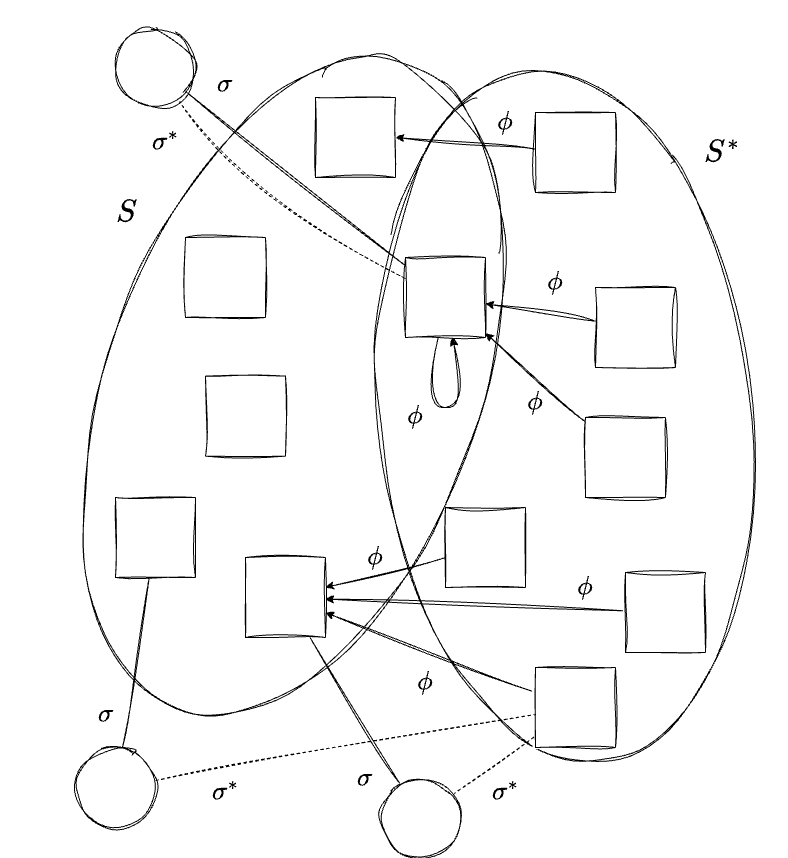
\includegraphics[width=1.0\textwidth]{figures/notation.drawio.png}
			\end{figure}
		\end{column}
	\end{columns}

	\note{
		\begin{itemize}
			\item 本発表では一貫して，施設を四角で，顧客を丸で表す
			\item \(S \bigcap S^*\) の施設に対しては，\(\phi\) は恒等写像になる
		\end{itemize}
	}

\end{frame}

\section{局所最適解の解析}

\begin{frame}{施設配置問題に対する局所最適解の性質}
	\begin{lemma}[割り当てコスト，\cite{korupolu2000analysis}]
		局所最適解 \(\localopt\) に対して，
		\(C \le F^* + C^* = \OPT\)
		が成立する．
	\end{lemma}

	\begin{lemma}[開設コスト，\cite{arya2004local}]
		局所最適解 \(\localopt\) に対して，
		\(F \le F^* + 2C^*\)
		が成立する．
	\end{lemma}

	\begin{theorem}[\cite{arya2004local}]
		施設配置問題の局所最適解 \(\localopt\) の総コストは，高々 \(3\OPT\) である．
	\end{theorem}

	\textbf{Proof. } 局所最適解の総コストは \(C + F\) であり，上の 2 つの補題より，
	\[C + F \le (F^* + C^*) + (F^* + 2C^*) = 2F^* + 3C^* \le 3F^* + 3C^* = 3\OPT.\]

	\note{
		\begin{itemize}
			\item 割り当てコストの上界は，削除操作／交換操作で解が改善する場合でさえ（追加操作でのみ改善しない解であったとしても），同様の不等式が成立する（より強いことがいえる）
			      \begin{itemize}
				      \item なお \cite{korupolu2000analysis} はこれの対偶を主張している
			      \end{itemize}
			\item \(2F^* + 3C^* \le 3F^* + 3C^*\) は大雑把な見積もりのように見えるが，ほぼほぼ近似比が \(3\) になるようなタイトな例が存在し，そこでは開設コストが \(0\) である
			      \begin{itemize}
				      \item インスタンスの開設コストと割り当てコストの比率を調整することで（ナップサック問題に対する FPTAS と同様にスケーリングと呼ばれる手法を用いて），この近似比を \(1 + \sqrt{2}\) まで改善できることを後ほど説明する
			      \end{itemize}
		\end{itemize}
	}
\end{frame}

\begin{frame}[label=tight-example]{施設配置問題に対する局所最適解のタイトな例}
	局所最適解の総コストが最適値の少なくとも \hyperlink{tight-example-analysis}{\(3 - o(1)\) 倍}になる例~(\cite{arya2004local})．
	\begin{figure}
		\centering
		
\includegraphics[width=0.85\textwidth]{figures/lower-bound.drawio.png}
	\end{figure}

	\note{
		\begin{itemize}
			\item まずインスタンスの説明（開設コスト \(0\) の施設が \(k+1\) 個，開設コスト \(2k\) の施設が \(1\) 個，顧客が \(k+1\) 人，すべての距離が \(1\) であること）
			\item 施設 \(i_0\) を開設し，各顧客をそれぞれの施設に割り当てる解のコストが \(2k + (k+1) = 3k + 1\) であること
			\item 追加操作，交換操作によって解の値が改善されないので，これは局所最適解であること
			\item 最適解は，施設 \(i_0\) 以外の施設をすべて開設し，各顧客をそれぞれの施設に割り当てる解であり，そのコストは \(k + 1\) であること
		\end{itemize}
	}
\end{frame}

\subsection{割り当てコストの上界}

\subsection{開設コストの上界}

\begin{frame}{準備：再割当てにおけるコストの増加分の上界}
	\begin{lemma}[再割当てにおけるコストの増加分の上界]
		\(\sigma(j) = i\) である利用者 \(j\) について，施設 \(i\) が \(i' = \phi(\sigma^*(j))\) と異なるとする．
		このとき，利用者 \(j\) を（施設 \(i\) から）施設 \(i'\) に再割り当てしたときのコストの増加分 (\(\alert{c_{i'j} - c_{ij}}\)) は，
		高々 \(\alert{2c_{\sigma^*(j)j}}\) である．
	\end{lemma}

	\vskip -1.5em

	\only<1>{
		\begin{figure}
			\centering
			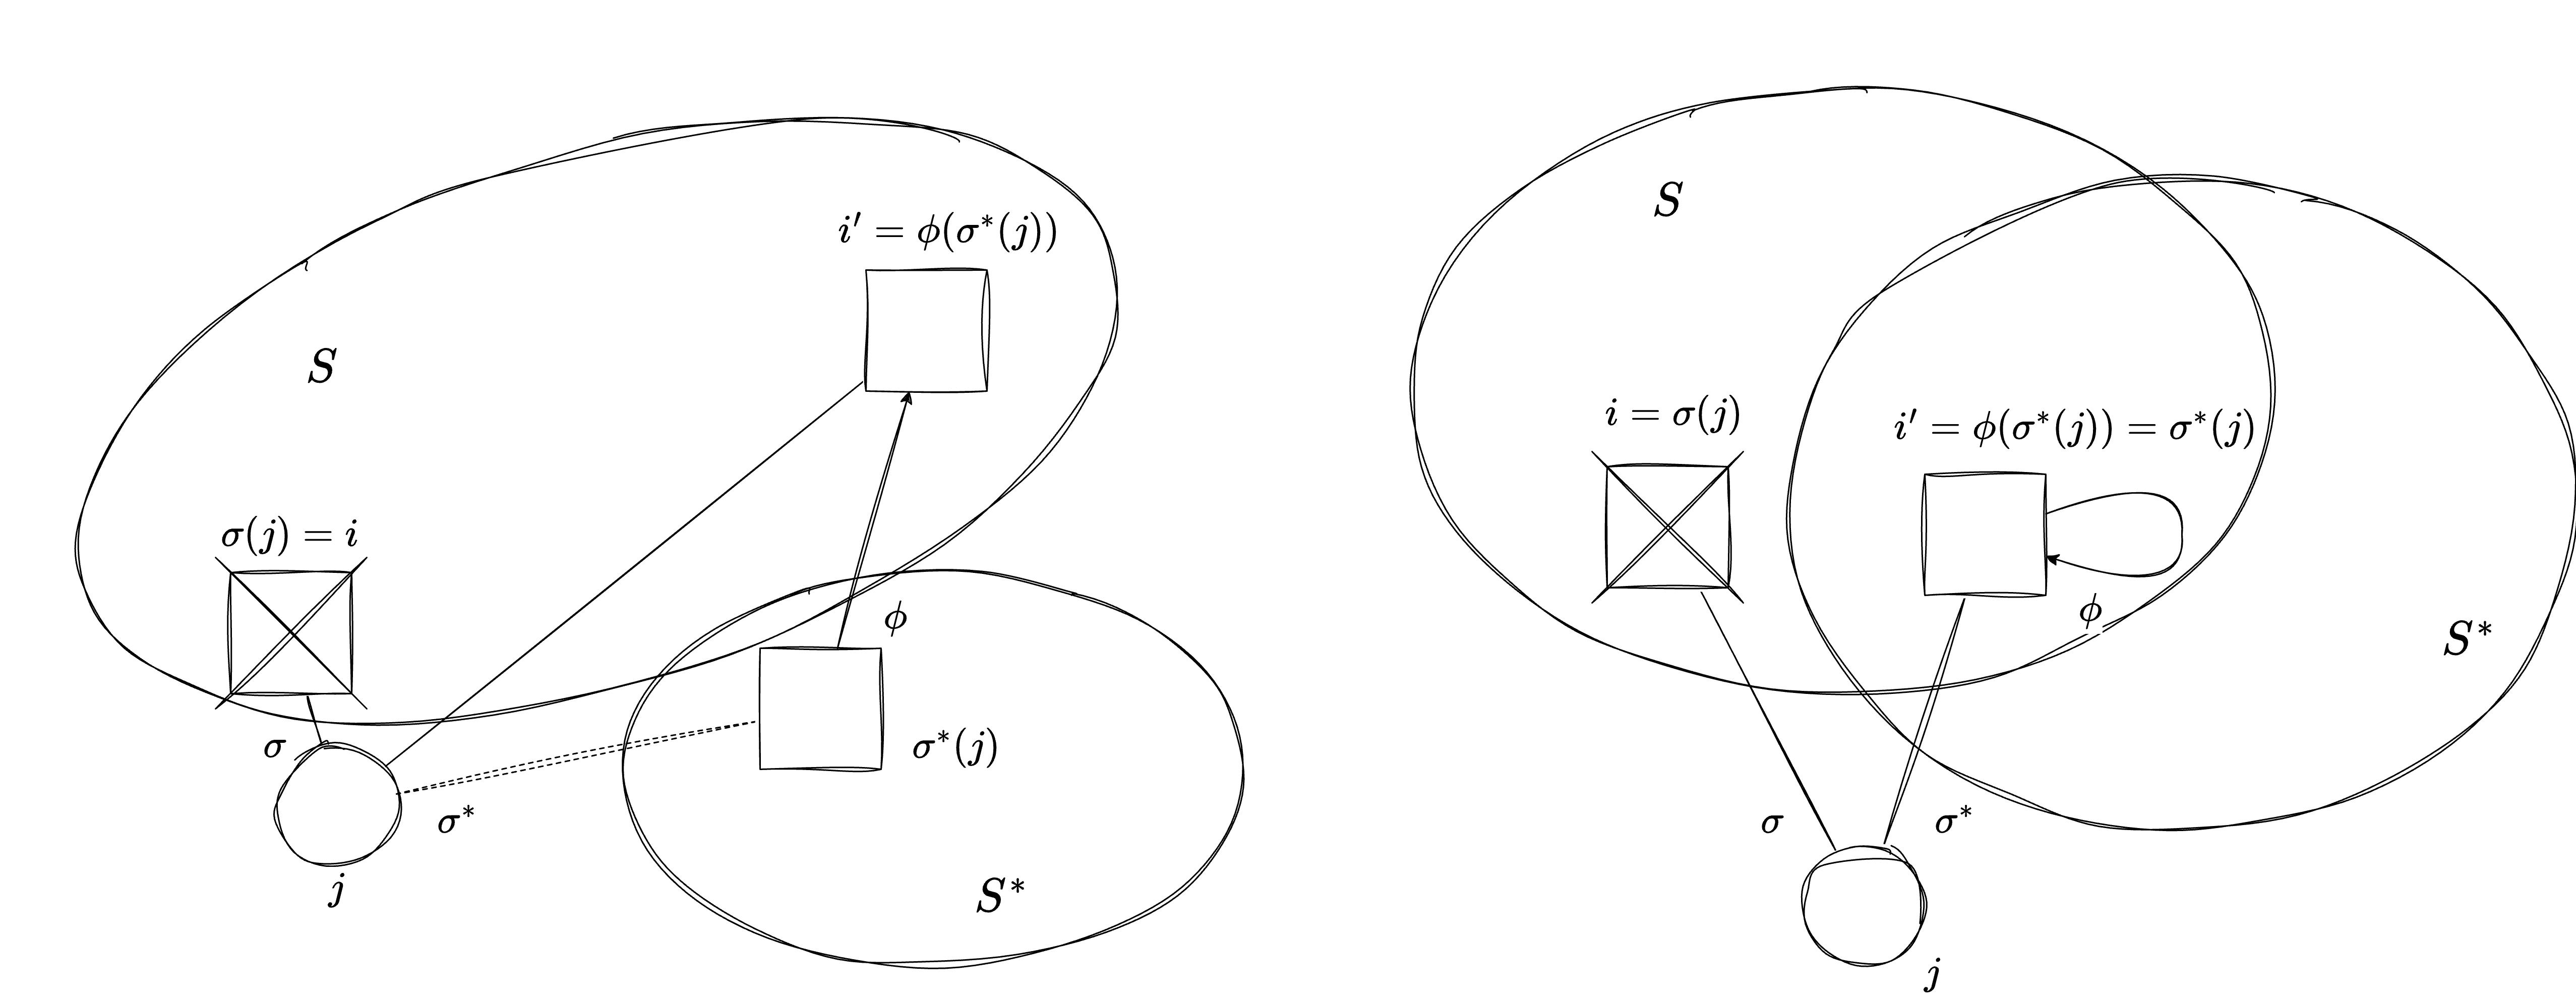
\includegraphics[width=0.9\textwidth]{figures/lemma7-9/possible-cases.drawio.png}
			\caption{左は \(c_{i'j} - c_{ij} \approx 2c_{\sigma^*(j)j}\) になる例．右のように \(S \bigcap S^*\) の施設が \(i'\) になる場合もある．}
		\end{figure}
	}
	\only<2->{
		\begin{columns}
			\begin{column}{0.5\textwidth}
				\begin{figure}
					\centering
					\only<2>{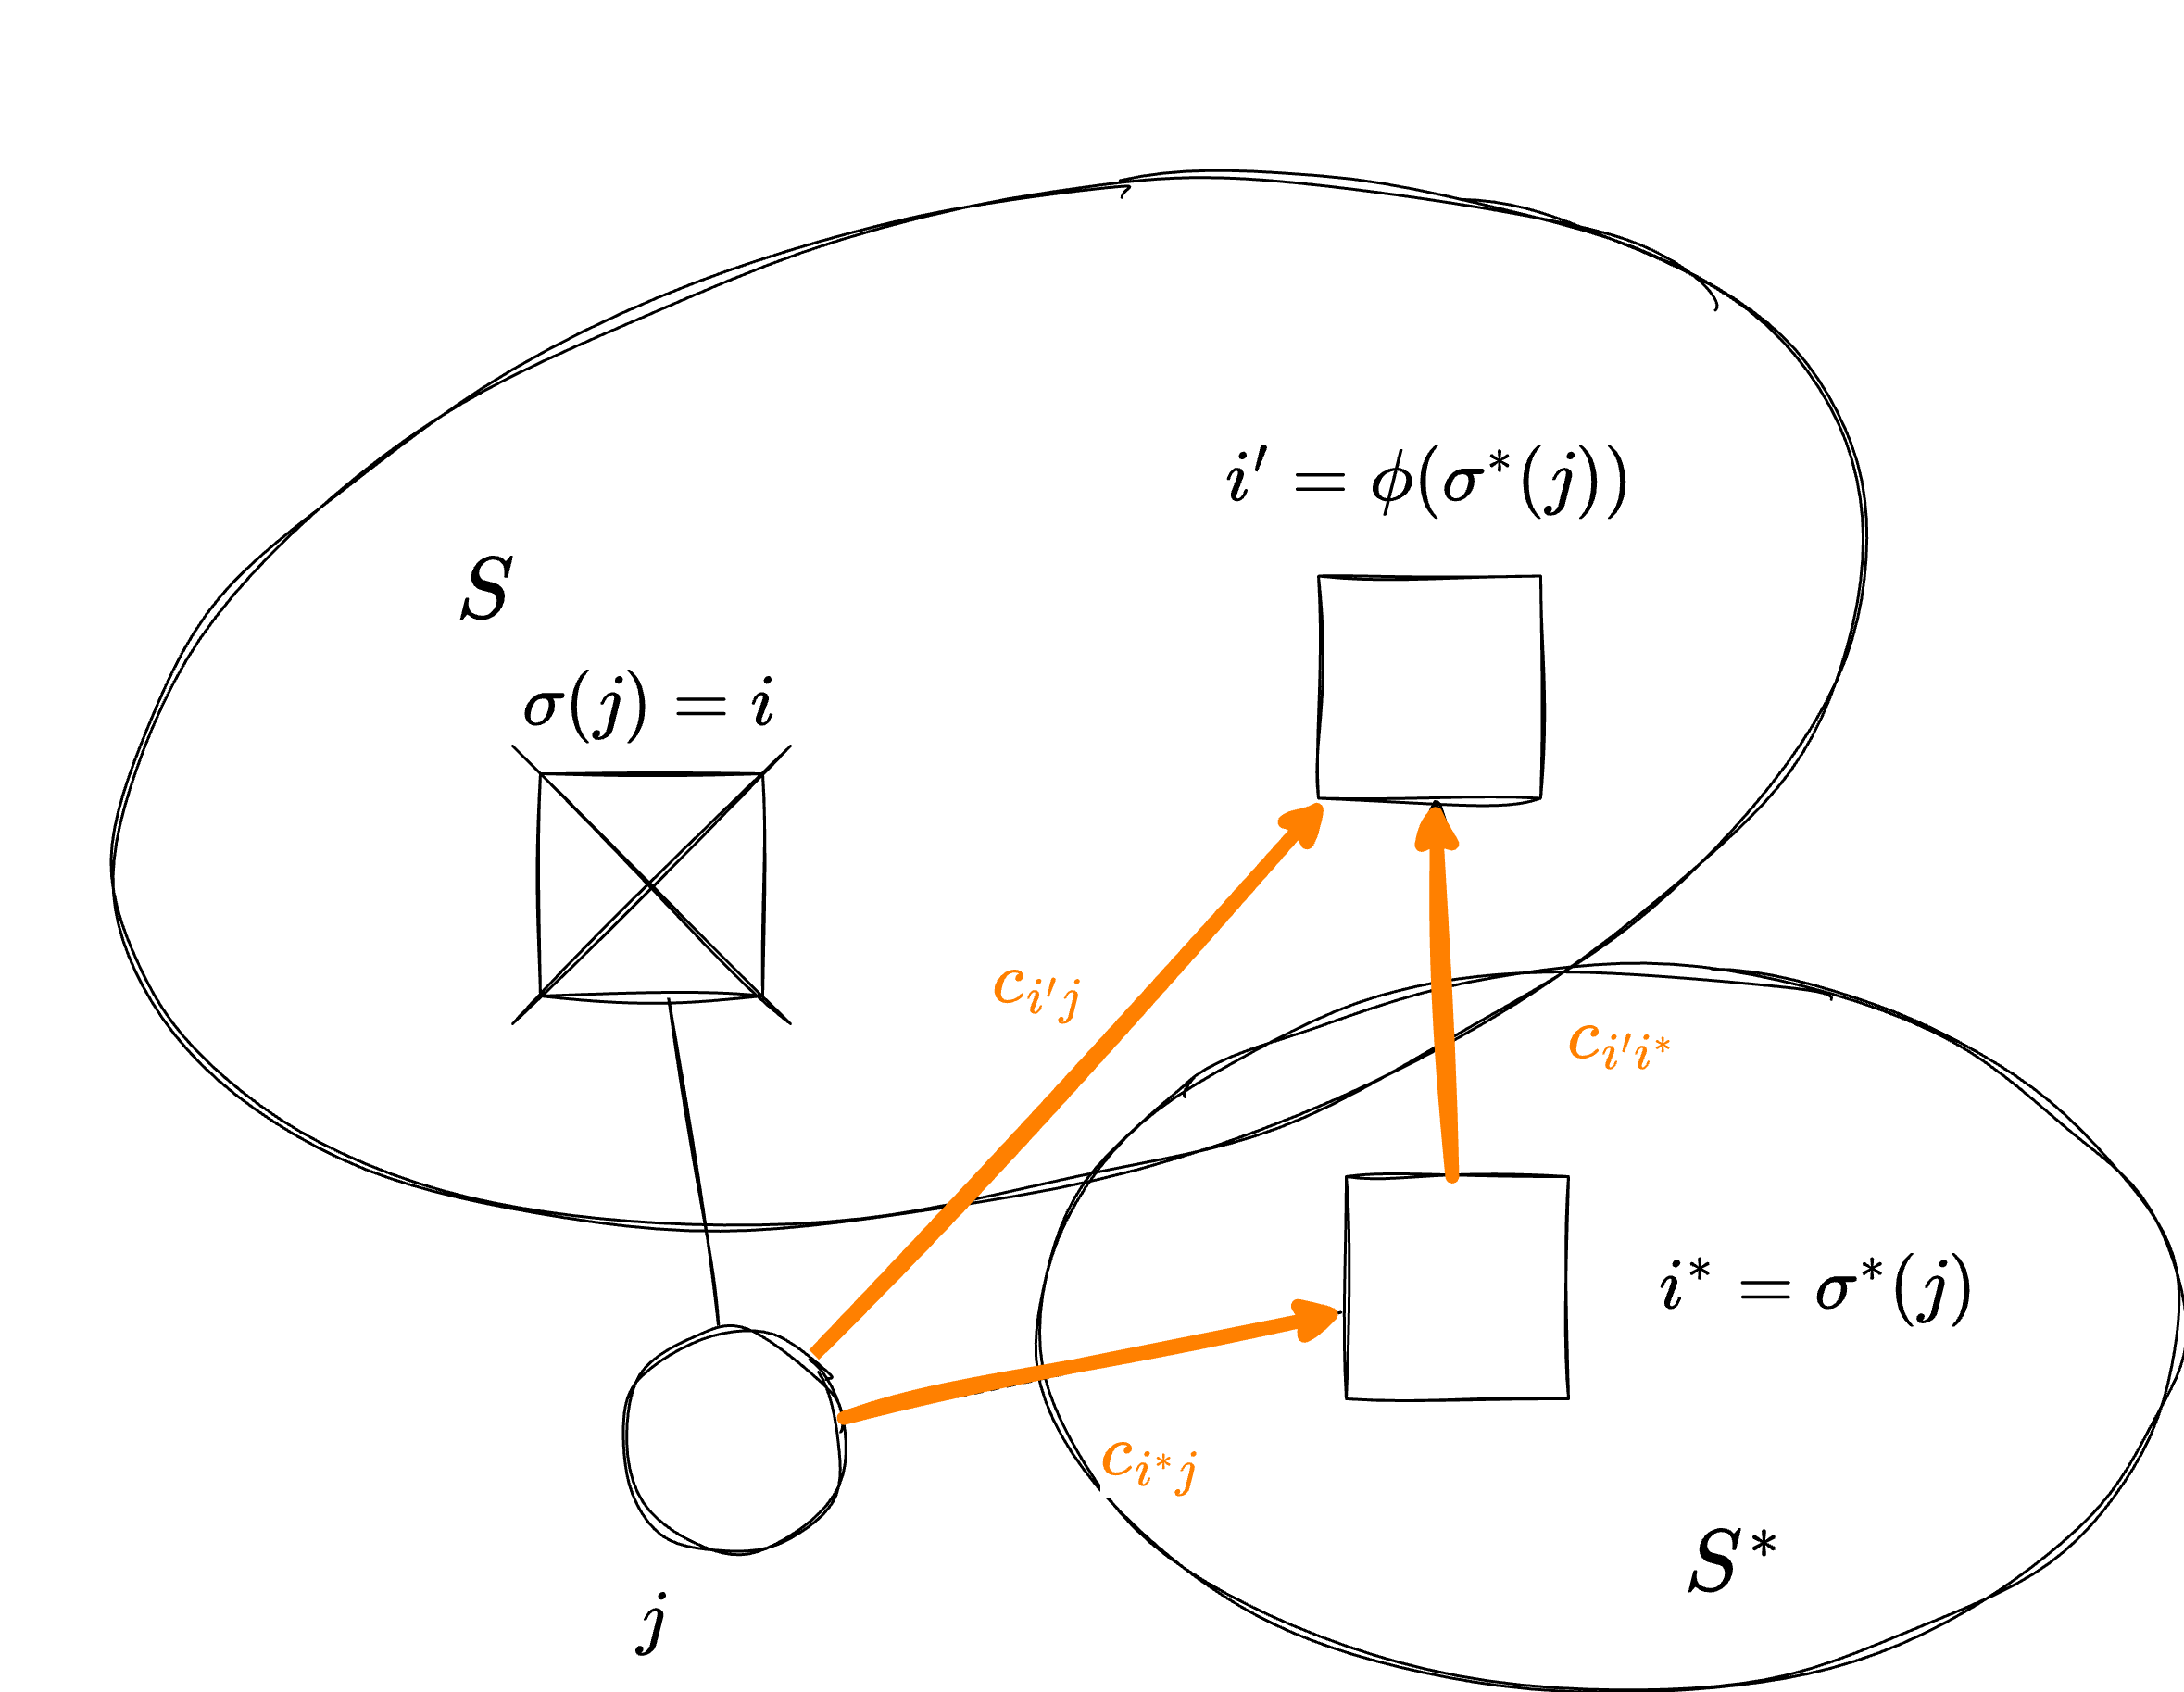
\includegraphics[width=0.9\textwidth]{figures/lemma7-9/proof-01.drawio.png}}
					\only<3>{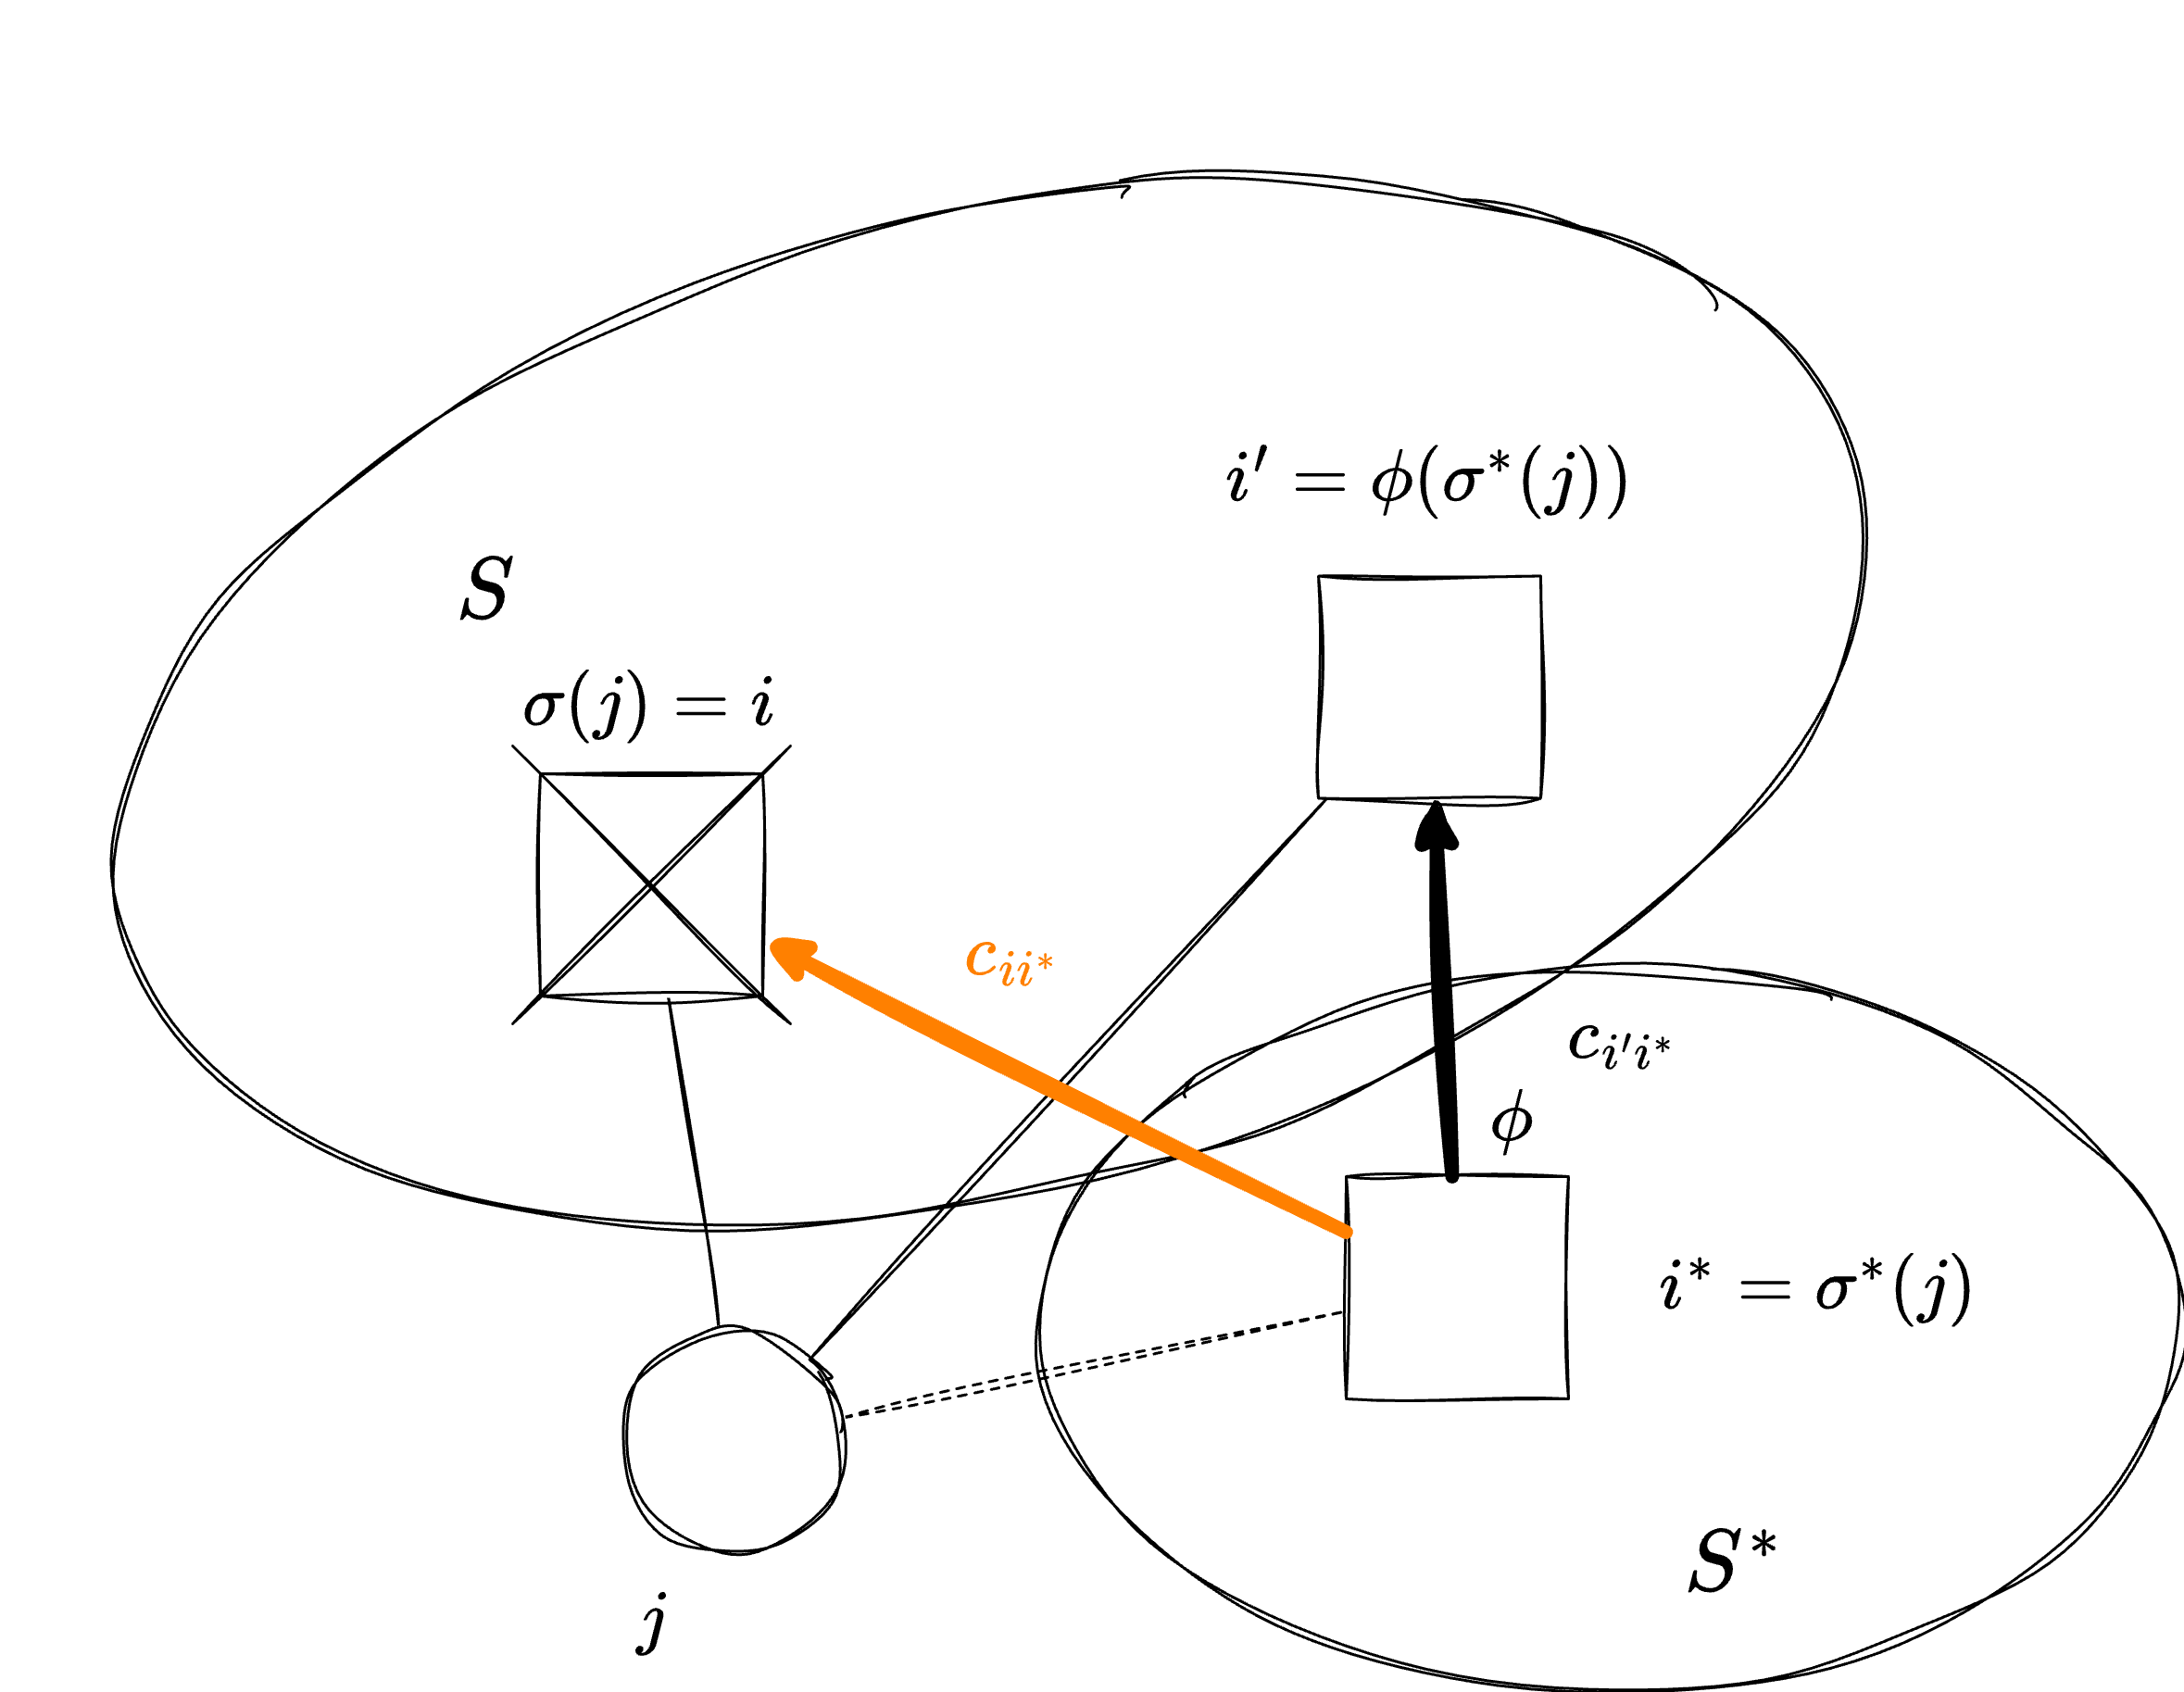
\includegraphics[width=0.9\textwidth]{figures/lemma7-9/proof-02.drawio.png}}
					\only<4>{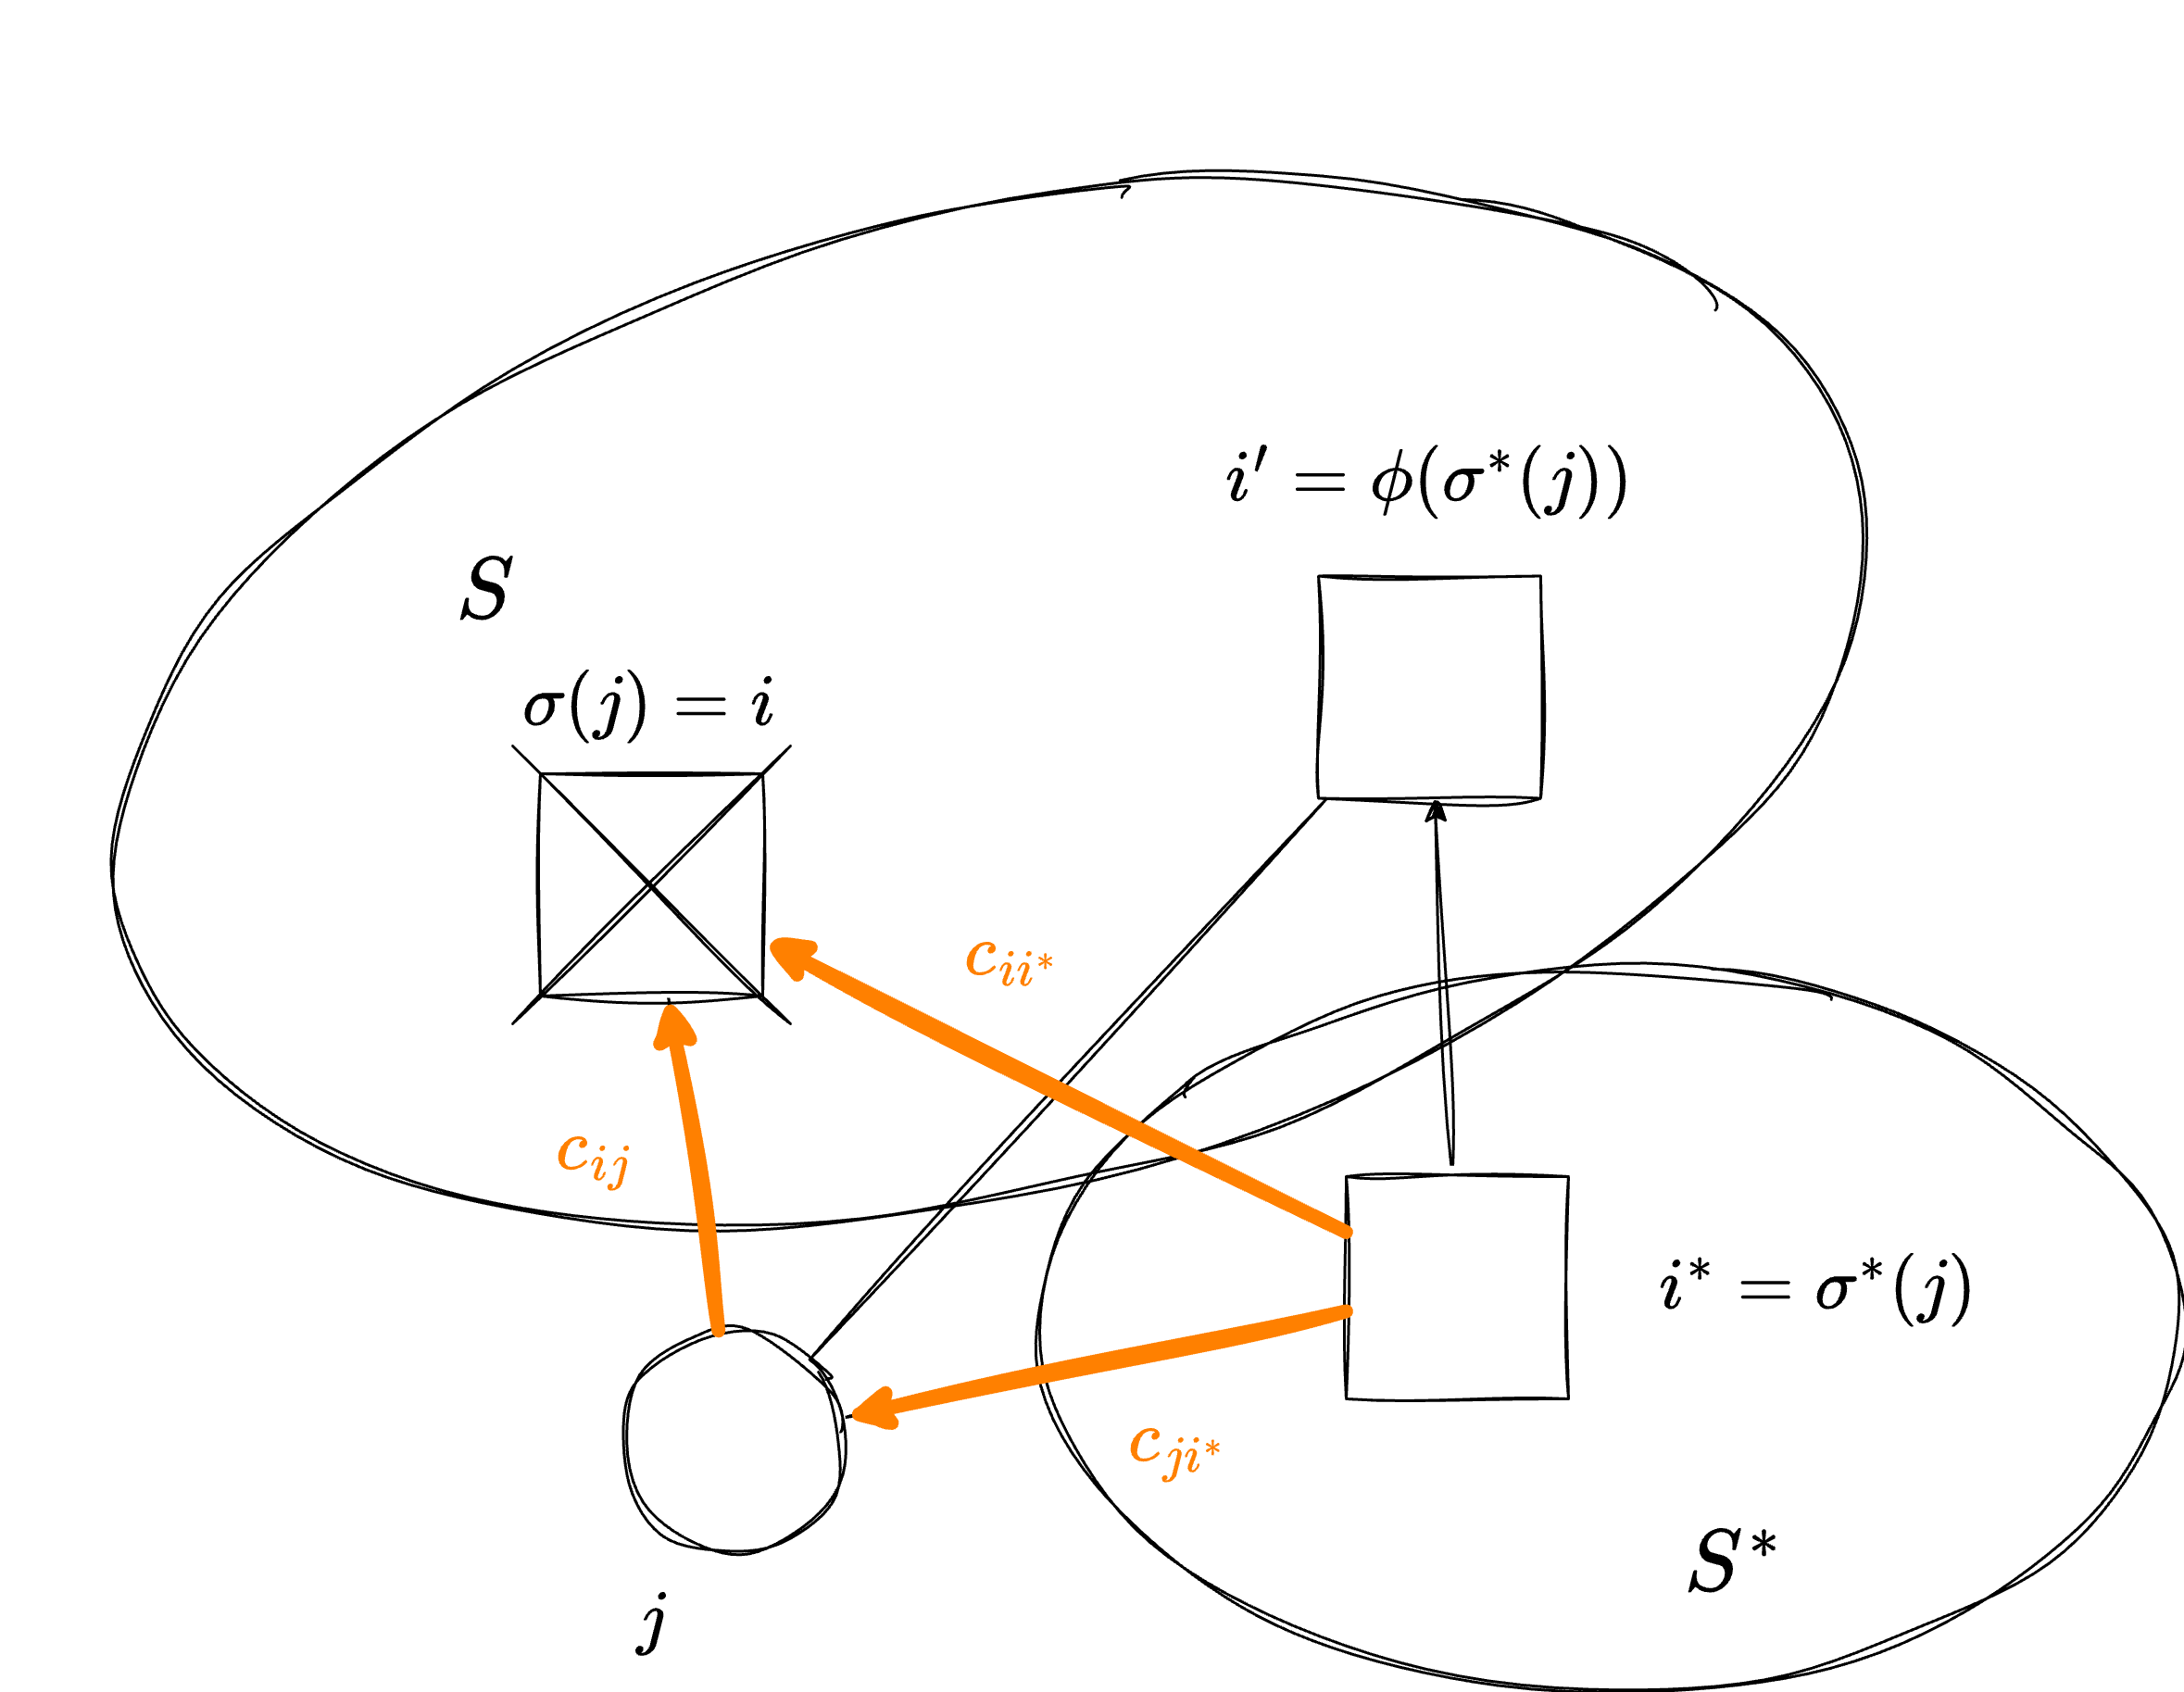
\includegraphics[width=0.9\textwidth]{figures/lemma7-9/proof-03.drawio.png}}
				\end{figure}
			\end{column}
			\begin{column}{0.5\textwidth}
				\vskip 1.5em

				\textbf{Proof. }
				\(i^* = \sigma^*(j)\) とする．\\
				三角不等式と \(\phi\) の定義から，
				\begin{align*}
					\uncover<2->{c_{i'j} & \le c_{i'\alert{i^*}} + c_{\alert{i^*}j}}           \\
					\uncover<3->{        & \le c_{\alert{i}i^*} + c_{i^*j}}                    \\
					\uncover<4->{        & \le (c_{i\alert{j}} + c_{\alert{j}i^*}) + c_{i^*j}}
				\end{align*}
				\uncover<4->{
					\(\qquad \Rightarrow \alert{c_{i'j} - c_{ij} \le 2c_{i^*j}}\).

					\hfill\(\qed\)
				}
			\end{column}
		\end{columns}
	}

	\note<1>{
		\begin{itemize}
			\item これから削除移動や交換移動を考えるが，今割り当てられている施設が閉じてしまった場合にどうするか少し予習
			\item \(j\) さんが次にサービスを受ける施設の決め方としてあり得るものは，最適解において割り当てられていた施設から最も近い施設に割り当て直す方法である（もちろんそのような施設が存在すれば）
			\item 直感的にはそこまで悪くなさそうで，実際にこの割り当ての変化によるコストの増加分は，三角不等式によって上界を与えることができるというのがこの補題
		\end{itemize}
		---
		\begin{itemize}
			\item ちなみに増加分と明記している通り，\(c_{i_{\unsafe}'j} - c_{ij}\) は必ず非負になることに注意（各利用者は開設集合に最も近い施設に割り当てられるので）
		\end{itemize}
	}

	\note<2>{
		\begin{itemize}
			\item 三角不等式
		\end{itemize}
	}

	\note<3>{
		\begin{itemize}
			\item \(\phi\) の定義（\(S\) の施設の中で最も \(i^*\) から近いのが \(i'\)）
		\end{itemize}
	}

	\note<4>{
		\begin{itemize}
			\item 三角不等式
			\item 距離関数の対称性を利用（\( c_{ji^*} = c_{i^*j}\)）
		\end{itemize}
	}
\end{frame}

\begin{frame}{開設コストの上界}
	\begin{lemma}[開設コスト，\cite{arya2004local}]
		局所最適解 \(\localopt\) に対して，
		\(F \le F^* + 2C^*\)
		が成立する．
	\end{lemma}

	\only<1>{
		\textbf{Key idea.}
		\structure{局所最適解の施設集合に対して施設を削除，（最適解の施設集合の施設を）追加・交換することによって得られる不等式を足し合わせる}

		\[
			\underbrace{
				\tikz[remember picture, baseline=(facility.base)]{
					\node[inner sep=0pt] (facility) { \text{(施設の開閉に伴うコストの変化)} };
				}
				+
				\tikz[remember picture, baseline=(assignment.base)]{
					\node[inner sep=0pt] (assignment) { \text{(割り当ての変化に伴うコストの変化)} };
				}
			}_{\text{局所最適解とその近傍解のコストの差}} \alert{\ge 0}
		\]

		\begin{tikzpicture}[remember picture, overlay, decoration=penciline,]
			\node[anchor=south] (facility-explain)
			at ([xshift=-0.5cm,yshift=-2.0cm] facility.south)
			{\(-f_i\) (削除), \(f_{i^*}\) (追加), \(-f_i + f_{i^*}\) (交換)};

			\draw[decorate, ->]
			(facility.south) -- (facility-explain.north);

			\node[anchor=south] (assignment-explain)
			at ([xshift=1cm,yshift=-2.0cm] assignment.south)
			{概ね \(2c_{\sigma^*(j)j}\) で上から抑えられる};

			\draw[decorate, ->]
			(assignment.south) -- (assignment-explain.north);

		\end{tikzpicture}
	}

	\only<2>{
		\textbf{Sketch of the Proof.}\footnote{本発表では \cite{gupta2008simpler} によって再構成された証明に基づいて説明する．}
		\begin{enumerate}
			\item \(S\) の各施設を（再割り当ての補題を即座に利用できるかという点で）\info{安全}，\alert{安全でない}施設に分類
			\item \info{安全}な各施設に対して削除移動を考え，\info{安全}な施設の開設コストの上界を得る
			      \tikz[remember picture, baseline]{
				      \node[inner sep=0pt] (ub-safe) {};
			      }
			\item \alert{安全でない}各施設に対して（対応する最適解の施設の／との）\\追加／交換移動を考え，\alert{安全でない}施設の開設コストの上界を得る
			      \tikz[remember picture, baseline]{
				      \node[inner sep=0pt] (ub-unsafe) {};
			      }
			\item 以上の上界を全て足し合わせて，開設コストの上界を得る
		\end{enumerate}

		\begin{columns}
			\begin{column}{0.4\textwidth}
				\begin{tikzpicture}[
						remember picture,
						baseline,
						box/.style={
								draw,
								rectangle,
								align=center,
								inner sep=6pt
							},
						decoration=penciline,
					]
					\node[decorate, box] (ineq-safe)
					{$
							f_{\isafe}
							\le
							\sum_{j \in D : \sigma(j)=\isafe} 2c_{\sigma^*(j)j}
						$};
				\end{tikzpicture}
			\end{column}
			\begin{column}{0.6\textwidth}
				\begin{tikzpicture}[
						remember picture,
						baseline,
						box/.style={
								draw,
								rectangle,
								align=center,
								inner sep=6pt
							},
						decoration=penciline,
					]
					\node[decorate, box] (ineq-unsafe)
					{$
							f_{\iunsafe}
							\le
							\sum_{i^* \in \phi^{-1}(\iunsafe)} f_{i^*}
							+ \sum_{j \in D : \sigma(j)=\iunsafe} 2c_{\sigma^*(j)j}
						$};
				\end{tikzpicture}
			\end{column}
		\end{columns}

		% % --- arrows ---
		% \begin{tikzpicture}[
		% 		remember picture,
		% 		overlay,
		% 	]
		% 	\draw[<-]
		% 	(ineq-safe.north)
		% 	to[bend right=15]
		% 	(ub-safe.south);

		% 	\draw[<-]
		% 	(ineq-unsafe.north)
		% 	to[bend right=15]
		% 	(ub-unsafe.south);
		% \end{tikzpicture}
	}
\end{frame}

\begin{frame}{準備：安全な施設と安全でない施設}
	\begin{columns}
		\begin{column}{0.45\textwidth}
			\begin{figure}
				\centering
				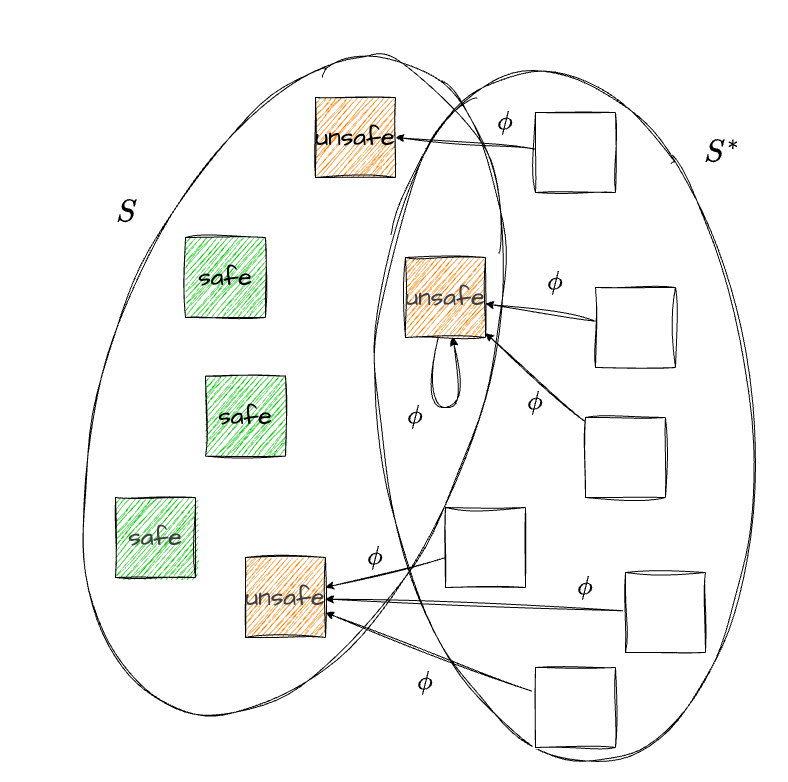
\includegraphics[width=\textwidth]{figures/safe-facility.drawio.png}
			\end{figure}
		\end{column}
		\begin{column}{0.45\textwidth}
			\begin{definition}[安全な施設]
				施設 \(i \in S\) が\info{安全}であるとは，
				最適解の全ての施設 \(i^* \in S^*\) について，
				\[
					\phi(i^*) \neq i
				\]
				が成立することである．つまり，\(\phi^{-1}(i) = \emptyset\) であることを意味する．
			\end{definition}
			逆に，ある施設 \(i^* \in S^*\) について，
			\[
				\phi(i^*) = i
			\]
			が成立する場合，施設 \(i\) を\alert{安全でない}とよぶ．
		\end{column}
	\end{columns}

	\note{
		\begin{itemize}
			\item 安全の意味は，その施設を削除した際に，元々その施設からサービスを受けていた利用者が，ある程度近い施設に再割り当てされることが保証されている，ということである
			\item \cite{asano2019} の定義とは異なり，利用者の割り当てを考慮せず，施設の位置関係のみに基づいて定義している（より強い）ことに注意
		\end{itemize}
	}
\end{frame}

\begin{frame}{\info{安全}な施設の開設コストの上界：削除移動による不等式の導出}
	\begin{columns}
		\begin{column}{0.45\textwidth}
			\begin{figure}
				\centering
				\only<1>{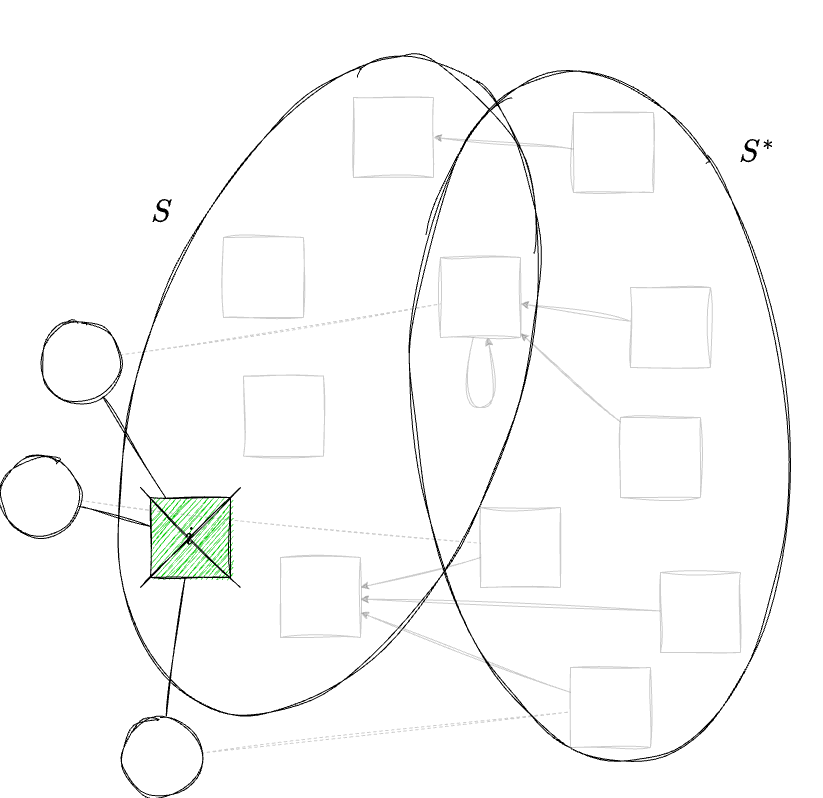
\includegraphics[width=\textwidth]{figures/lemma7-10/drop-01.drawio.png}}
				\only<2->{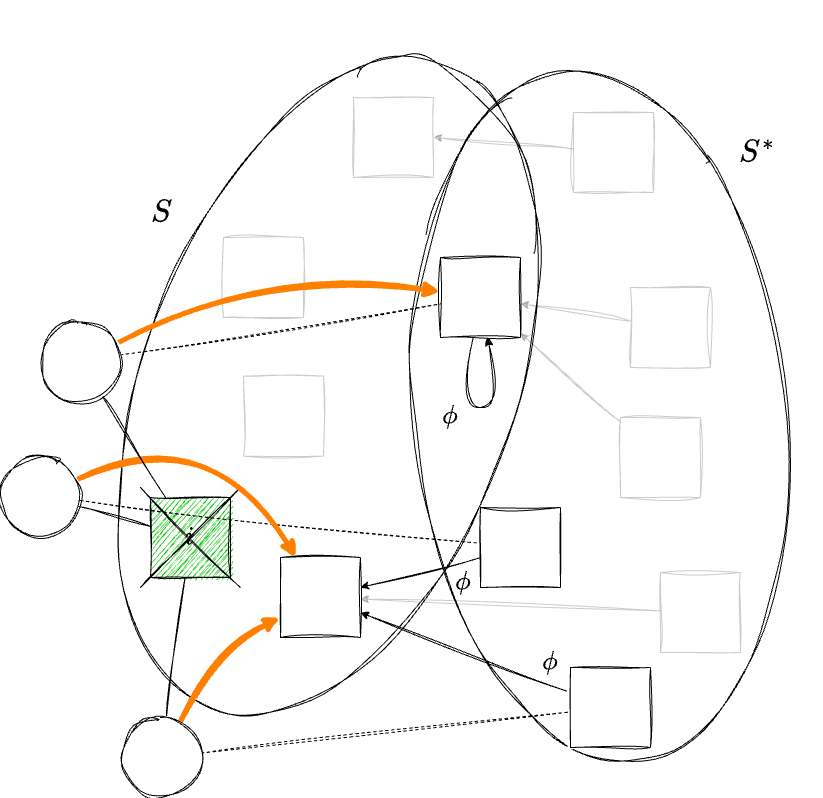
\includegraphics[width=\textwidth]{figures/lemma7-10/drop-02.drawio.png}}
			\end{figure}
		\end{column}

		\begin{column}{0.50\textwidth}
			\only<1-2>{
				\begin{itemize}
					\item \info{安全}な施設 \(\isafe \in S\) を一つ選び削除
					\item 局所最適解において \(\isafe\) に割り当てられていた各利用者\\ \(j: \sigma(j) = \isafe\) について， \\
					      \uncover<2>{
						      \(\qquad\qquad\qquad \Downarrow\) \\
						      最適解において \(j\) が割り当てられていた施設 \( \sigma^*(j) \) に最も近い \(S\) の施設 \(\alert{\phi(\sigma^*(j))}\) (\(\neq \info{i}\)) に割り当てる

						      \begin{block}{\info{安全}の定義}
							      \vskip -1em
							      \[
								      i \text{ が\info{安全} }
								      \;\stackrel{\text{def}}{\Longleftrightarrow}\;
								      \forall i^* \in S^*,\; \phi(i^*) \neq i
							      \]
							      \vskip -0.5em
						      \end{block}
					      }
				\end{itemize}
			}
			\small{
				\only<3->{
					\vskip 0.5em
					次式が得られる：
					\begin{align*}
						 & \underbrace{\sum_{i \in S} f_i + \sum_{j \in \DemandSet} c_{\sigma(j)j}}_{\text{局所最適解 } (S, \sigma) \text{ のコスト}}                                                                                                                                           \\
						 & \left(\le \underbrace{S - \{\isafe\} \text{ の下で最適な割り当てをした解のコスト}}_{(S, \sigma) \text{ の近傍解のコスト}}\right)                                                                                                                                                      \\
						 & \le \underbrace{\sum_{i \in S \setminus \{\isafe\}} f_i + \sum_{j \in \DemandSet \colon \sigma(j) \neq \isafe} c_{\sigma(j)j} + \sum_{j \in \DemandSet \colon \sigma(j) = \isafe} \alert{c_{\phi(\sigma^*(j))j}}}_{(S, \sigma) \text{ の近傍解の割り当てをいじった解のコスト}} \\
					\end{align*}
					\vskip -4.5em
				}
				\only<4->{
					\begin{align*}
						\Rightarrow f_{\isafe} & \le \sum_{j \in \DemandSet \colon \sigma(j) = \isafe} (c_{\phi(\sigma^*(j))j} - c_{\sigma(j)j})                  \\
						                       & \le \sum_{j \in \DemandSet \colon \sigma(j) = \isafe} \alert{2c_{\sigma^*(j)j}} \qquad \because{\text{再割り当ての補題}}
					\end{align*}
				}
			}
		\end{column}
	\end{columns}

	\note<2>{
		\begin{itemize}
			\item \(\isafe\) に割り当てられていない利用者の割り当ては変更しない
		\end{itemize}
	}

	\note<4>{
		\begin{itemize}
			\item 最後の不等式は，先ほどの補題を利用している
			\item 安全な各施設に対して，対応する利用者の最適解における割り当てコストを用いた上界が得られた．
		\end{itemize}
	}
\end{frame}

\begin{frame}{\alert{安全でない}施設の開設コストの上界：施設に対応する最適解の施設集合}
	\begin{columns}
		\begin{column}{0.40\textwidth}
			\begin{figure}
				\centering
				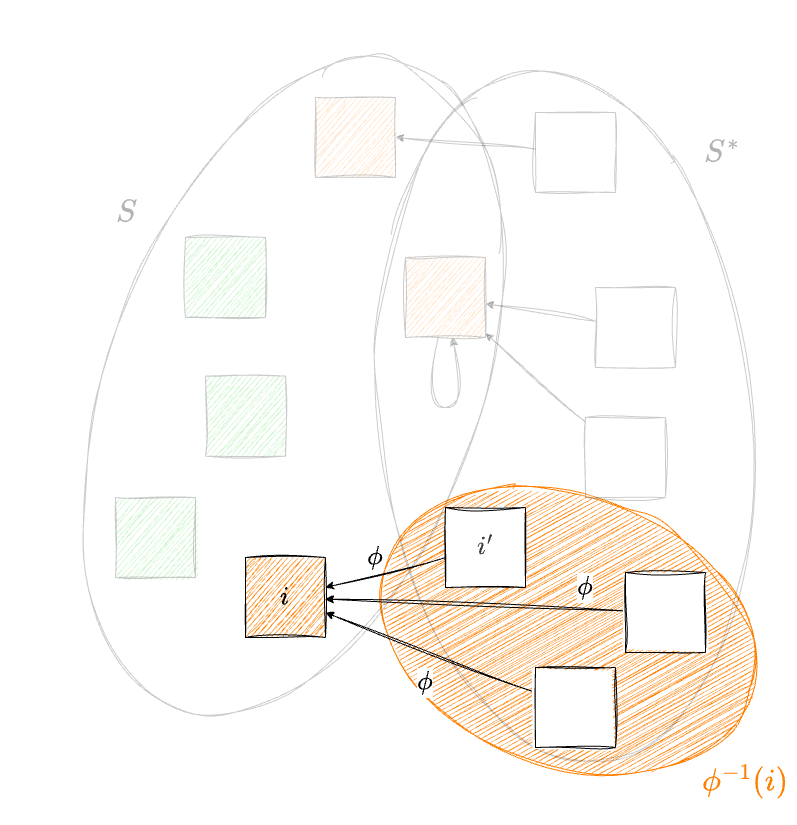
\includegraphics[width=\textwidth]{figures/corresponding-facilities-of-unsafe-i.drawio.png}
			\end{figure}
		\end{column}
		\begin{column}{0.50\textwidth}
			\begin{block}{\alert{安全でない}の定義}
				\(i\) が\alert{安全でない} \(\;\stackrel{\text{def}}{\Longleftrightarrow}\;\)
				\(\exists i^* \in S^*,\; \phi(i^*) = \iunsafe\)
			\end{block}

			\begin{itemize}
				\item \alert{安全でない}施設 \(\iunsafe\) を固定
				\item \(\iunsafe\) に対し \(i'\) を定義
				      \begin{align*}
					      i' \coloneq \argmin_{\alert{i^*} \in \phi^{-1}(i)} c_{\alert{i^*} i}
				      \end{align*}
			\end{itemize}

			\vskip -1em

			\begin{block}{今後の展開}
				\begin{itemize}
					\item \(\phi^{-1}(i) \setminus {i'}\) の\alert{各施設の追加移動}，\\\(i\) と \(i'\) の\alert{交換移動}を考える
					\item 得られた \(|\phi^{-1}(i)|\) 個の不等式を\alert{足し合わせ}，\(i\) の開設コストの上界を得る
				\end{itemize}
			\end{block}
		\end{column}
	\end{columns}

	\note{
		\begin{itemize}
			\item 局所最適解の施設に追加／交換する最適解集合の施設の部分集合を考える
			\item \(\iunsafe\) に最も近い \(\phi^{-1}(\iunsafe)\) の施設を \(i'\) とする
		\end{itemize}
	}
\end{frame}

\begin{frame}{\alert{安全でない}施設の開設コストの上界：追加移動による不等式の導出}
	\begin{columns}
		\begin{column}{0.40\textwidth}
			\begin{figure}
				\centering
				\only<1>{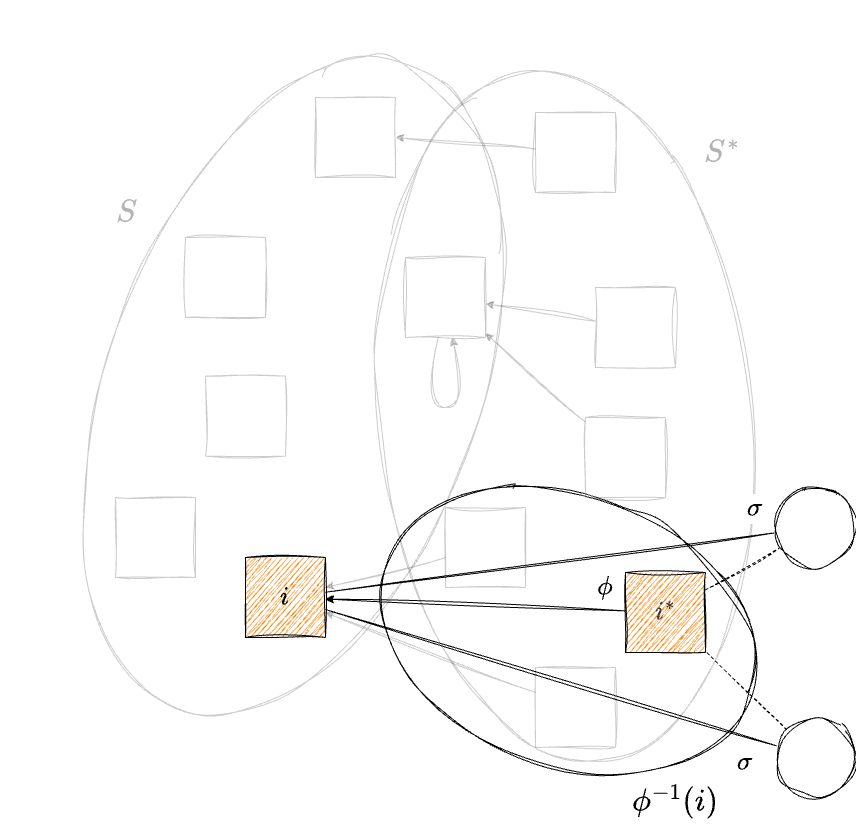
\includegraphics[width=\textwidth]{figures/lemma7-10/add-01.drawio.png}}
				\only<2->{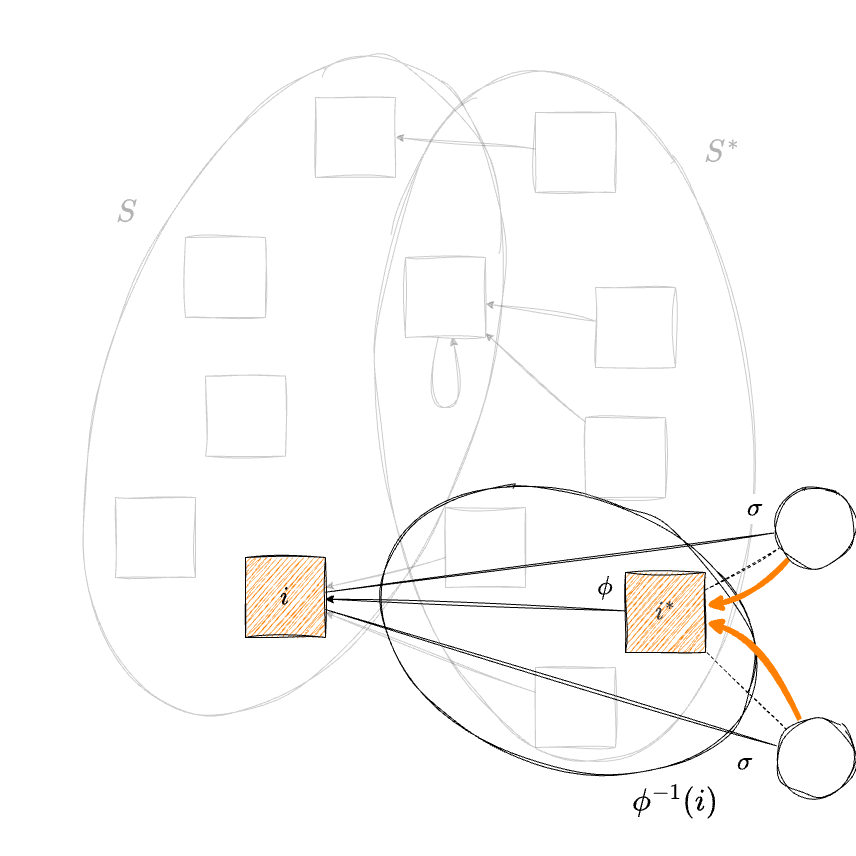
\includegraphics[width=\textwidth]{figures/lemma7-10/add-02.drawio.png}}
			\end{figure}
		\end{column}
		\begin{column}{0.50\textwidth}

			\only<1-2>{
				\begin{itemize}
					\item 施設 \(\alert{i^{*}} \in {\phi^{-1}(\alert{i}) \setminus \{i'\}}\) を開設
					\item 局所最適解において \(\iunsafe\) に，\\さらに最適解において \(\alert{i^*}\) に\\割り当てられていた各利用者\\ \(j: \sigma(j) = \iunsafe \text{ and } \sigma^*(j) = \alert{i^*}\) について， \\
					      \uncover<2>{
						      \(\qquad\qquad\qquad \Downarrow\) \\
						      \(\alert{i}\) から \(\alert{i^*}\) に割り当てる
					      }
				\end{itemize}
			}
			\small{
				\only<3->{
					\only<3>{
						\vskip 0.5em
						次式が得られる：
					}
					\begin{align*}
						 & \underbrace{\sum_{i \in S} f_i + \sum_{j \in \DemandSet} c_{\sigma(j)j}}_{\text{局所最適解 } (S, \sigma) \text{ のコスト}}                                                                                                                                \\
						 & \left(\le \underbrace{S \cup \{i^{*}\} \text{ の下で最適な割り当てをした解のコスト}}_{(S, \sigma) \text{ の近傍解のコスト}}\right)                                                                                                                                         \\
						 & \underbrace{\begin{aligned} \le \sum_{i \in S \cup \{i^{*}\}} f_i & + \sum_{j \in \DemandSet \colon \overline{\sigma(j) = \iunsafe \text{ and } \sigma^*(j) = i^{*}}} c_{\sigma(j)j} \\
                                                      & + \sum_{j \in \DemandSet \colon \sigma(j) = \iunsafe \text{ and } \sigma^*(j) = i^{*}} \alert{c_{\sigma^*(j)j}}
							               \end{aligned}}_{(S, \sigma) \text{ の近傍解の割り当てをいじった解のコスト}} \\
					\end{align*}
					\vskip -4.5em
				}
				\only<4>{
					\begin{align*}
						\Rightarrow 0 & \le f_{i^*} + \sum_{j \in \DemandSet \colon \sigma(j) = \iunsafe \text{ and } \sigma^*(j) = i^{*}} (c_{\sigma^*(j)j} - c_{\sigma(j)j}) \\
					\end{align*}
				}
			}
		\end{column}
	\end{columns}
\end{frame}

\begin{frame}[plain, noframenumbering]{【再掲】\alert{安全でない}施設の開設コストの上界：施設に対応する最適解の施設集合}
	\begin{columns}
		\begin{column}{0.40\textwidth}
			\begin{figure}
				\centering
				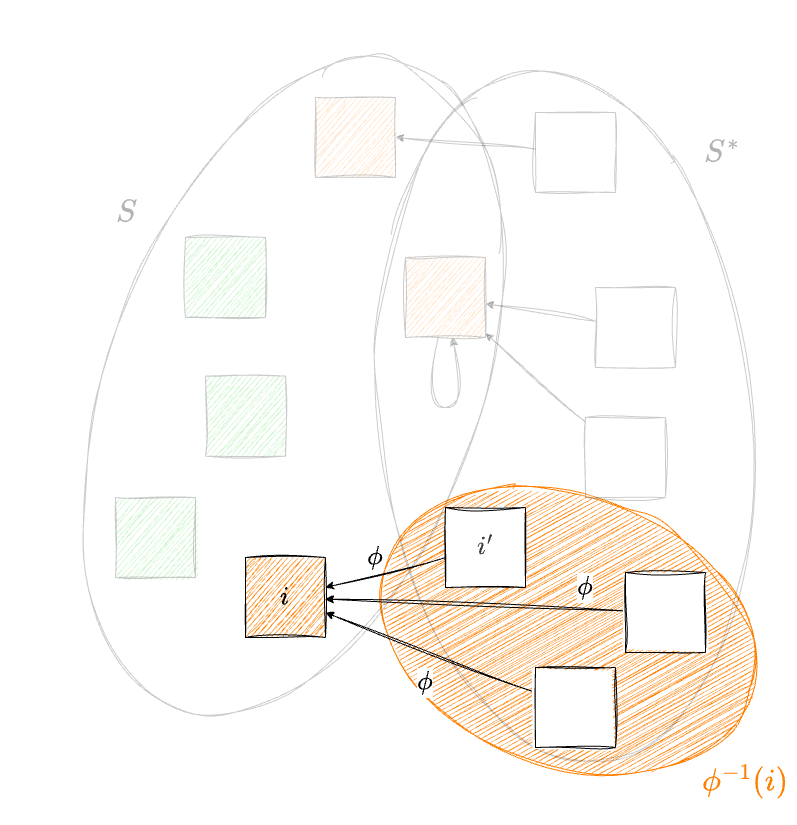
\includegraphics[width=\textwidth]{figures/corresponding-facilities-of-unsafe-i.drawio.png}
			\end{figure}
		\end{column}
		\begin{column}{0.50\textwidth}
			\begin{block}{\alert{安全でない}の定義}
				\(i\) が\alert{安全でない} \(\;\stackrel{\text{def}}{\Longleftrightarrow}\;\)
				\(\exists i^* \in S^*,\; \phi(i^*) = \iunsafe\)
			\end{block}

			\begin{itemize}
				\item \alert{安全でない}施設 \(\iunsafe\) を固定
				\item \(\iunsafe\) に対し \(i'\) を定義
				      \begin{align*}
					      i' \coloneq \argmin_{\alert{i^*} \in \phi^{-1}(i)} c_{\alert{i^*} i}
				      \end{align*}
			\end{itemize}

			\vskip -1em

			\begin{block}{今後の展開}
				\begin{itemize}
					\item \(\phi^{-1}(i) \setminus {i'}\) の\alert{各施設の追加移動}，\\\(i\) と \(i'\) の\alert{交換移動}を考える \(\leftarrow\text{next}\)
					\item 得られた \(|\phi^{-1}(i)|\) 個の不等式を\alert{足し合わせ}，\(i\) の開設コストの上界を得る
				\end{itemize}
			\end{block}
		\end{column}
	\end{columns}

	\note{
		\begin{itemize}
			\item
		\end{itemize}
	}
\end{frame}

\begin{frame}{\alert{安全でない}施設の開設コストの上界：交換移動による不等式の導出}
	\begin{columns}
		\begin{column}{0.45\textwidth}
			\begin{figure}
				\centering
				\only<1>{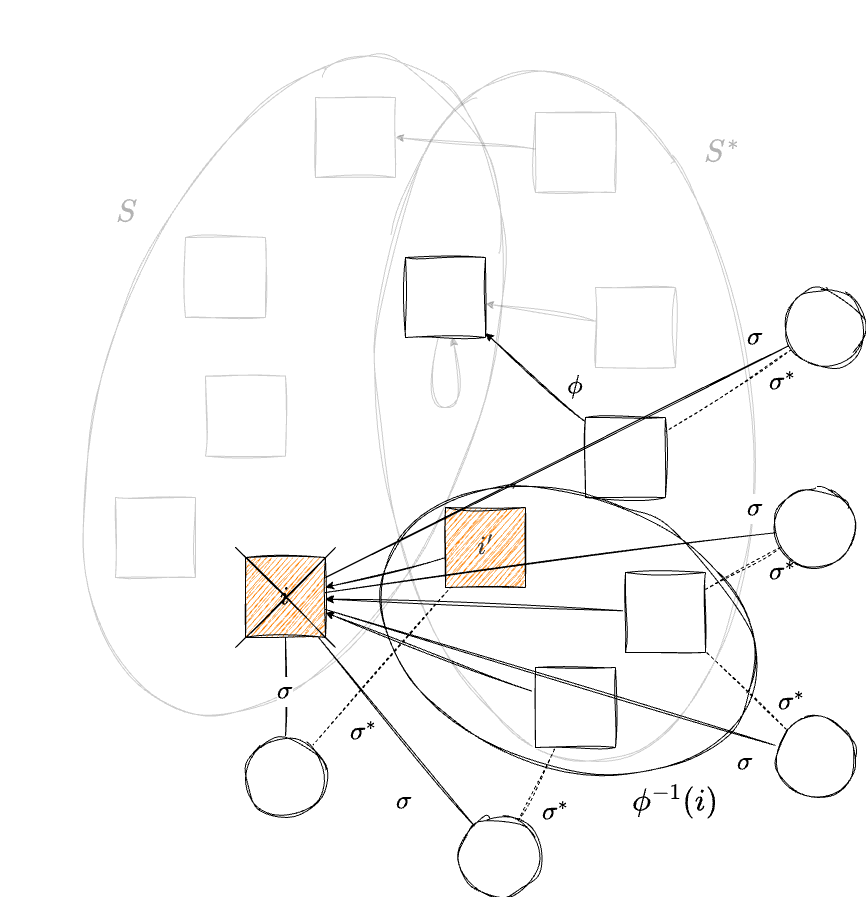
\includegraphics[width=\textwidth]{figures/lemma7-10/swap-01.drawio.png}}
				\only<2->{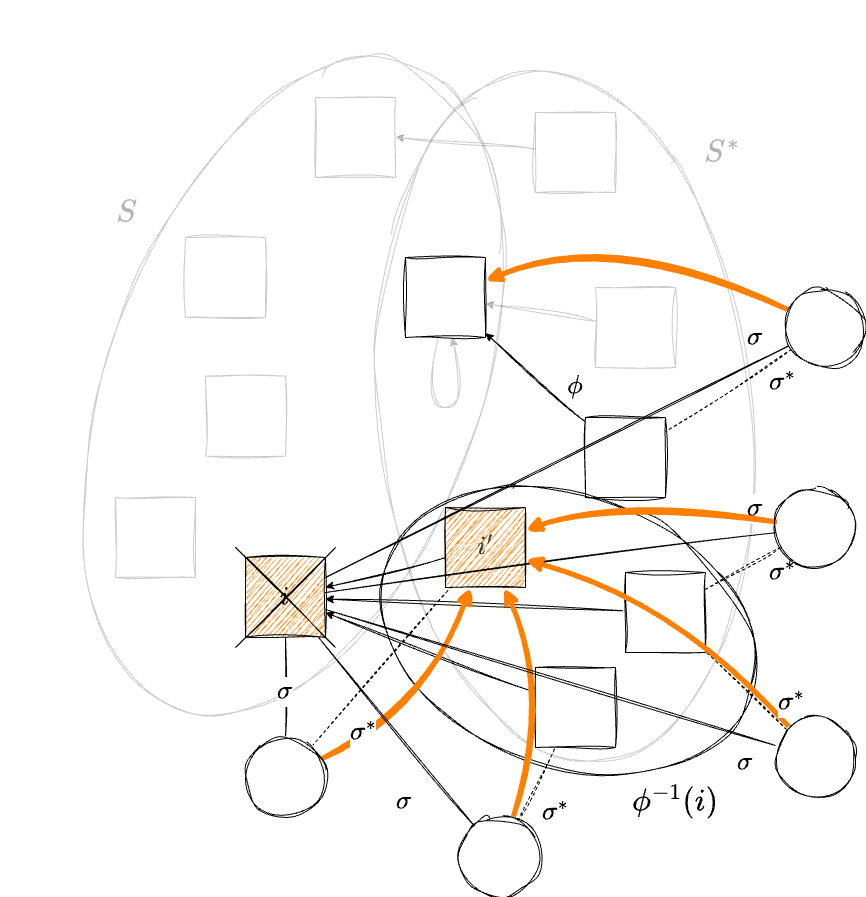
\includegraphics[width=\textwidth]{figures/lemma7-10/swap-02.drawio.png}}
			\end{figure}
		\end{column}
		\begin{column}{0.50\textwidth}
			\only<1-2>{
				\begin{itemize}
					\item \(\iunsafe\) を閉鎖し，施設 \(i'\) を開設
					\item 局所最適解において \(\iunsafe\) に割り当てられていた各利用者\\ \(j: \sigma(j) = \iunsafe\) について，
					      \begin{itemize}
						      \item<2> \(\sigma^*(j) \in \phi^{-1}(\iunsafe)\) であれば，\\\(j\) を \(i'\) に割り当てる
						      \item<2> \(\sigma^*(j) \notin \phi^{-1}(\iunsafe)\) であれば，\\\(j\) を \(\phi(\sigma^*(j))\) (\(\neq \iunsafe\)) に割り当てる
						            \tikz[remember picture, baseline]{
							            \node[inner sep=0pt] (R-unsafe) {};
						            }
					      \end{itemize}
				\end{itemize}
				\uncover<2>{
					\begin{tikzpicture}
						\draw[->]
						(R-unsafe.east)
						to[bend right=40]
						([yshift=1em] R-unsafe.east);
						\node[anchor=east] at (R-unsafe.east)
						{\small{再割り当て補題が適用できる利用者}};
					\end{tikzpicture}

					\begin{block}{定義の言い換え}
						\(\sigma^*(j) \in \phi^{-1}(\iunsafe) \iff \phi(\sigma^*(j)) = \iunsafe\)
					\end{block}
				}
			}
			\small{
				\only<3>{
					\begin{align*}
						 & \underbrace{\sum_{i \in S} f_i + \sum_{j \in \DemandSet} c_{\sigma(j)j}}_{\text{局所最適解 } (S, \sigma) \text{ のコスト}}                                                                     \\
						 & \left(\le \underbrace{S \cup \{i'\} \setminus \{\iunsafe\} \text{ の下で最適な割り当てをした解のコスト}}_{(S, \sigma) \text{ の近傍解のコスト}}\right)                                                          \\
						 & \underbrace{\begin{aligned}
								               \le \sum_{i \in S \cup \{i'\} \setminus \{\iunsafe\}} f_i
								                & + \sum_{j \in D \colon \sigma(j) \neq \iunsafe} c_{\sigma(j)j}                                                          \\
								                & + \sum_{j \in D \colon \sigma(j) = \iunsafe \text{ and } \sigma^*(j) \in \phi^{-1}(\iunsafe)} c_{i'j}                   \\
								                & + \sum_{j \in D \colon \sigma(j) = \iunsafe \text{ and } \sigma^*(j) \notin \phi^{-1}(\iunsafe)} c_{\phi(\sigma^*(j))j}
							               \end{aligned}}_{(S, \sigma) \text{ の近傍解の割り当てをいじった解のコスト}} \\
					\end{align*}
				}
				\only<4>{
					\begin{align*}
						\Rightarrow f_{\iunsafe} & \le \begin{aligned}[t]
							                               f_{i'}
							                                & + \sum_{j \in D \colon \sigma(j) = \iunsafe \text{ and } \sigma^*(j) \in \phi^{-1}(\iunsafe)} (c_{i'j} - c_{\sigma(j)j})                   \\
							                                & + \sum_{j \in D \colon \sigma(j) = \iunsafe \text{ and } \sigma^*(j) \notin \phi^{-1}(\iunsafe)} (c_{\phi(\sigma^*(j))j} - c_{\sigma(j)j})
						                               \end{aligned} \\
						                         & \le \begin{aligned}[t]
							                               f_{i'}
							                                & + \sum_{j \in D \colon \sigma(j) = \iunsafe \text{ and } \sigma^*(j) \in \phi^{-1}(\iunsafe)} (c_{i'j} - c_{\sigma(j)j})   \\
							                                & + \sum_{j \in D \colon \sigma(j) = \iunsafe \text{ and } \sigma^*(j) \notin \phi^{-1}(\iunsafe)} \alert{2c_{\sigma^*(j)j}}
							                                & \qquad\qquad\qquad \because{\text{再割り当ての補題}}
						                               \end{aligned}
					\end{align*}
				}
			}
		\end{column}
	\end{columns}

	\note<1>{
		\begin{itemize}
			\item 当然 \(i \neq i'\) でないと交換移動にならないが，後に得られる不等式は \(i = i'\) の場合にも成立するので問題ない
			\item 各利用者 \(j: \sigma(j) = \iunsafe\) について，全員再割り当てを行う
		\end{itemize}
	}

	\note<2>{
		\begin{itemize}
			\item 基本的には \(\phi(\sigma^*(j))\) に割り当て直す
			\item \(\phi(\sigma^*(j))\) が今閉じた施設 \(\iunsafe\) である場合は（つまり，\(\sigma^*(j) \in \phi^{-1}(i)\) の場合は）\(i'\) に割り当てる
		\end{itemize}
	}

	\note<3>{
		\begin{itemize}
			\item ここまでがあまり理解できてないと \(c_{i_{\unsafe}'j} - c_{\phi(j)j}\) はそのまま放置するんですか？という疑問が出るかもしれない
			\item 他の場合と異なり，\(i_{\unsafe}'\) への割り当て\(c_{\sigma^*(j)j}\) の定数倍で抑えられる保証がないからというのが端的な回答
		\end{itemize}
	}

	\note<4>{
		\begin{itemize}
			\item \(c_{i'j}\) がちょっと邪魔だが後でうまく処理する
		\end{itemize}
	}
\end{frame}

\begin{frame}{\alert{安全でない}施設の開設コストの上界：不等式の足し合わせ (1/3)}

	\begin{columns}
		\begin{column}{0.45\textwidth}
			\begin{figure}
				\centering
				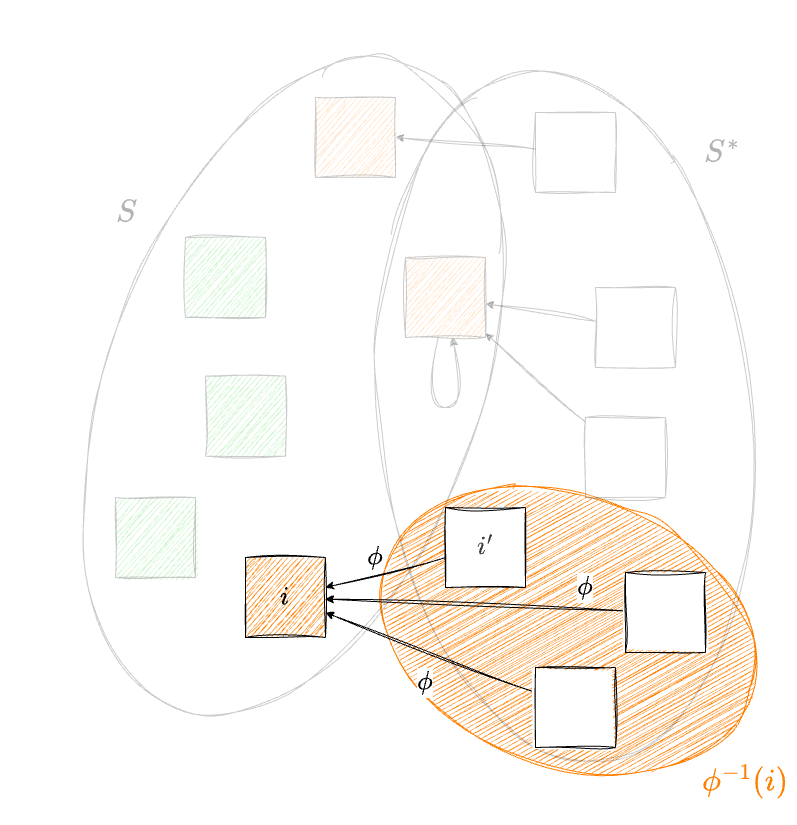
\includegraphics[width=\textwidth]{figures/corresponding-facilities-of-unsafe-i.drawio.png}
			\end{figure}
		\end{column}
		\begin{column}{0.5\textwidth}
			\vskip 1em

			\small{
				\structure{各 \(i^* \in \phi^{-1}(\iunsafe)\setminus \{i'\}\) に対する追加移動で}
				\begin{align*}
					0 & \le f_{i^*} + \sum_{j \in \DemandSet \colon \sigma(j) = \iunsafe \text{ and } \sigma^*(j) = i^{*}} (c_{\sigma^*(j)j} - c_{\sigma(j)j}) \\
				\end{align*}

				\vskip -1em

				\structure{\(\iunsafe\) と \(i'\) に対する交換移動で}
				\begin{align*}
					f_{\iunsafe} & \le \begin{aligned}[t]
						                   f_{i'}
						                    & + \sum_{j \in D \colon \sigma(j) = \iunsafe \text{ and } \sigma^*(j) \in \phi^{-1}(\iunsafe)} (c_{i'j} - c_{\sigma(j)j}) \\
						                    & + \sum_{j \in D \colon \sigma(j) = \iunsafe \text{ and } \sigma^*(j) \notin \phi^{-1}(\iunsafe)} 2c_{\sigma^*(j)j}
					                   \end{aligned}
				\end{align*}

				得た，計 \(|\phi^{-1}(\iunsafe)|\) 個の不等式を足し合わせる．
			}
		\end{column}
	\end{columns}

	\note{
		\begin{itemize}
			\item 後少し．頑張ろう
		\end{itemize}
	}
\end{frame}

\begin{frame}{\alert{安全でない}施設の開設コストの上界：不等式の足し合わせ (2/3)}

	\begin{align*}
		f_{i} \le & \sum_{i^* \in \phi^{-1}(i) \setminus \{i'\}} \biggl(f_{i^*} + \sum_{j \in \DemandSet \colon \sigma(j) = i \text{ and } \sigma^*(j) = i^{*}} (c_{\sigma^*(j)j} - c_{\sigma(j)j})\biggr)                                                                                                                  \\
		          & + \begin{aligned}[t]
			              f_{i'}
			               & + \sum_{j \in D \colon \sigma(j) = i \text{ and } \sigma^*(j) \in \phi^{-1}(i)} (c_{i'j} - c_{\sigma(j)j}) \\
			               & + \sum_{j \in D \colon \sigma(j) = i \text{ and } \sigma^*(j) \notin \phi^{-1}(i)} 2c_{\sigma^*(j)j}
		              \end{aligned}                                                                                                                            \\
		=         & \sum_{i^* \in \alert{\phi^{-1}(i)}} f_{i^*} \begin{aligned}[t]
			                                                         & + \sum_{j \in \DemandSet \colon \sigma(j) = i \text{ and } \sigma^*(j) \alert{\in \phi^{-1}(i) \setminus \{i'\}}} (c_{\sigma^*(j)j} - c_{\sigma(j)j}) \qquad \because{i' \in \phi^{-1}(i)} \\
			                                                         & + \sum_{j \in D \colon \sigma(j) = i \text{ and } \sigma^*(j) \in \phi^{-1}(i)} (c_{i'j} - c_{\sigma(j)j})                                                                                 \\
			                                                         & + \sum_{j \in D \colon \sigma(j) = i \text{ and } \sigma^*(j) \notin \phi^{-1}(i)} 2c_{\sigma^*(j)j}
		                                                        \end{aligned} \\
	\end{align*}

	\note{
		\begin{itemize}
			\item まず開設コストの項をまとめる（必ず \(i'\) は \(\phi^{-1}(i)\) に含まれるため，等号変形が可能．さもなければ左辺の方が大きくなる）
			\item 次に二重和の項を一重和にまとめる
		\end{itemize}
	}
\end{frame}

\begin{frame}{\alert{安全でない}施設の開設コストの上界：不等式の足し合わせ (3/3)}
	\small{
		中央の二項の和に注目すると，
		\begin{align*}
			                  & \sum_{j \colon \sigma(j) = i \text{ and } \sigma^*(j) \in \phi^{-1}(i) \setminus\{i'\}} (c_{\sigma^*(j)j} - c_{\sigma(j)j}) + \sum_{j \colon \sigma(j) = i \text{ and } \sigma^*(j) \in \phi^{-1}(i)} (c_{i'j} - c_{\sigma(j)j})                                                                                        \\
			=                 & \sum_{j \colon \sigma(j) = i \text{ and } \alert{\sigma^*(j) \in \phi^{-1}(i) \setminus\{i'\}}} (c_{\sigma^*(j)j} + c_{i'j} - 2c_{\sigma(j)j}) + \sum_{j \colon \sigma(j) = i \text{ and } \alert{\sigma^*(j) = i'}} (c_{i'j} - c_{\sigma(j)j})                                                                         \\
			\uncover<2->{	\le & \sum_{j \colon \sigma(j) = i \text{ and } \sigma^*(j) \in \phi^{-1}(i) \setminus\{i'\}} (c_{\sigma^*(j)j} + \alert{(c_{\sigma^*(j)j} + 2c_{\sigma(j)j})} - 2c_{\sigma(j)j}) + \sum_{j \colon \sigma(j) = i \text{ and } \sigma^*(j) = i'} \alert{2c_{\sigma^*(j)j}} \\}
			\uncover<5>{=     & \sum_{j \colon \sigma(j) = i \text{ and } \sigma^*(j) \in \phi^{-1}(i) \setminus\{i'\}} 2c_{\sigma^*(j)j} + \sum_{j \colon \sigma(j) = i \text{ and } \sigma^*(j) = i'} 2c_{\sigma^*(j)j}                                                                                                     \\}
			\uncover<5>{=     & \sum_{j \colon \sigma(j) = i \text{ and } \sigma^*(j) \in \phi^{-1}(i)} 2c_{\sigma^*(j)j}}
		\end{align*}

		\uncover<5>{
			最終的に次式を得る．
			\(f_{i} \le \sum_{i^* \in \phi^{-1}(i)} f_{i^*} + \sum_{j \colon \sigma(j) = i \text{ and } \sigma^*(j) \in \phi^{-1}(i)} 2c_{\sigma^*(j)j} + \sum_{j \colon \sigma(j) = i \text{ and } \sigma^*(j) \notin \phi^{-1}(i)} 2c_{\sigma^*(j)j} \)
		}
	}

	\only<2-4>{
		\begin{tikzpicture}[
				remember picture,
				overlay,
				box/.style={
						draw,
						rectangle,
					},
				decoration=penciline,
			]
			\node[
				decorate,
				box,
				anchor=south east,
				fill=white,
				thick,
				inner sep=6pt,
				text width=0.6\linewidth
			] at ([xshift=-20pt,yshift=10pt]current page.south east)
			{
				\small
				\begin{minipage}{0.55\linewidth}


					\only<2>{
						\(c_{i'j}\) について，
						三角不等式より
						\[
							c_{i'j} \le c_{i'\alert{\sigma(j)}} + c_{\alert{\sigma(j)}j}
						\]
					}
					\only<3>{\(i'\) の定義より
						\begin{align*}
							c_{i'j} & \le c_{i'\sigma(j)} + c_{\sigma(j)j}                  \\
							        & \le c_{\alert{\sigma^*(j)}\sigma(j)} + c_{\sigma(j)j} \\
						\end{align*}
					}
					\only<4>{再度三角不等式より
						\begin{align*}
							c_{i'j} & \le c_{i'\sigma(j)} + c_{\sigma(j)j}                                     \\
							        & \le c_{\sigma^*(j)\sigma(j)} + c_{\sigma(j)j}                            \\
							        & \le (c_{\sigma^*(j)\alert{j}} + c_{\alert{j}\sigma(j)}) + c_{\sigma(j)j} \\
						\end{align*}
					}
				\end{minipage}
				\hfill
				\begin{minipage}{0.40\linewidth}
					\centering
					\only<2>{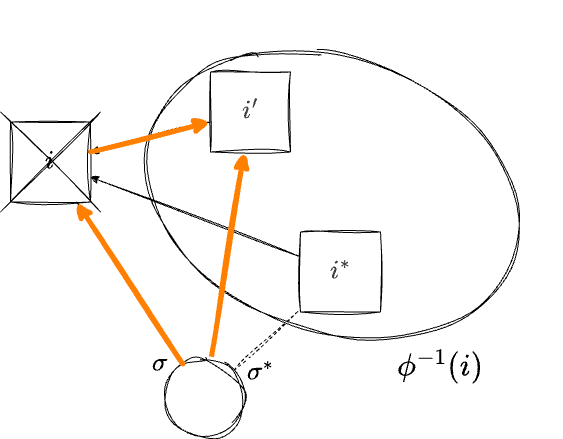
\includegraphics[width=\linewidth]{figures/lemma7-10/triangle-inequality-01.drawio.png}}
					\only<3>{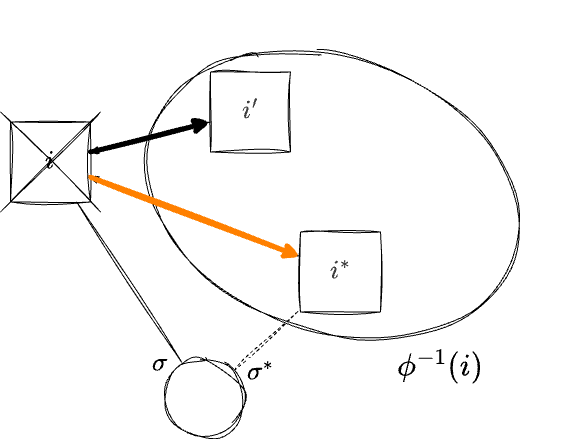
\includegraphics[width=\linewidth]{figures/lemma7-10/triangle-inequality-02.drawio.png}}
					\only<4>{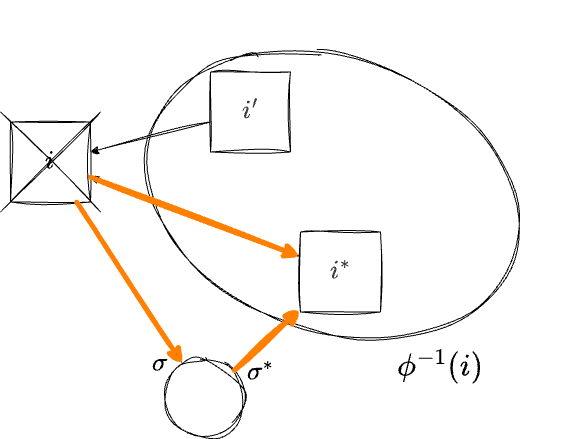
\includegraphics[width=\linewidth]{figures/lemma7-10/triangle-inequality-03.drawio.png}}
				\end{minipage}
			};
		\end{tikzpicture}

	}

	\note<1>{
		\begin{itemize}
			\item \(\sum_{j \colon \sigma(j) = i \text{ and } \sigma^*(j) \in \phi^{-1}(i)} \) の和を，\(\sigma^*(j) = i'\) とそれ以外に分けたもの
			\item 次の不等式について，
			      \begin{itemize}
				      \item \(c_{i'j} \le c_{i'\sigma(j)} + c_{\sigma(j)j} \le c_{\sigma^*(j)\sigma(j)} + c_{\sigma^(j)j} \le (c_{\sigma^*(j)j} + c_{j\sigma(j)}) + c_{\sigma(j)j} = c_{\sigma^*(j)j} + 2c_{\sigma(j)j}\) に関しては三角不等式と \(i'\) の定義を用いる
				      \item \(c_{i'j} - c_{\sigma(j)j} \le 2c_{\sigma^*(j)j}\) に関してはシンプルに \(c_{i'j} - c_{\sigma(j)j} \le c_{i'j} \le 2c_{i'j} = 2c_{\sigma^*(j)j}\)
			      \end{itemize}
		\end{itemize}
	}

	\note<2-4>{
		\begin{itemize}
			\item \(c_{i'j} - c_{\sigma(j)j} \le 2c_{\sigma^*(j)j}\) に関してはシンプルに \(c_{i'j} - c_{\sigma(j)j} \le c_{i'j} \le 2c_{i'j} = 2c_{\sigma^*(j)j}\)
		\end{itemize}
	}
\end{frame}

\begin{frame}{開設コストの上界}

	\info{安全}な各施設に対して
	\[f_{\isafe} \le \sum_{j \in \DemandSet \colon \sigma(j) = \isafe} 2c_{\sigma^*(j)j}\]
	\alert{安全でない}各施設に対して，
	\[\hfill f_{\iunsafe} \le \sum_{i^* \in \phi^{-1}(\iunsafe)} f_{i^*} + \sum_{j \in D \colon \sigma(j) = \iunsafe} 2c_{\sigma^*(j)j}\]

	以上の上界を \(S\) の各施設について全て足し合わせることで，補題が得られる．
	\hfill\qed

	\begin{lemma}[開設コスト，\cite{arya2004local}]
		局所最適解 \(\localopt\) に対して，
		\(F \le F^* + 2C^*\)
		が成立する．
	\end{lemma}

	\note{
		\begin{itemize}
			\item \(i\) が安全なとき \(\phi^{-1}(i)\) は空集合であるから，かなり美しい
		\end{itemize}
	}
\end{frame}
